% Options for packages loaded elsewhere
\PassOptionsToPackage{unicode}{hyperref}
\PassOptionsToPackage{hyphens}{url}
%
\documentclass[
  12pt,
]{article}
\usepackage{lmodern}
\usepackage{amssymb,amsmath}
\usepackage{ifxetex,ifluatex}
\ifnum 0\ifxetex 1\fi\ifluatex 1\fi=0 % if pdftex
  \usepackage[T1]{fontenc}
  \usepackage[utf8]{inputenc}
  \usepackage{textcomp} % provide euro and other symbols
\else % if luatex or xetex
  \usepackage{unicode-math}
  \defaultfontfeatures{Scale=MatchLowercase}
  \defaultfontfeatures[\rmfamily]{Ligatures=TeX,Scale=1}
\fi
% Use upquote if available, for straight quotes in verbatim environments
\IfFileExists{upquote.sty}{\usepackage{upquote}}{}
\IfFileExists{microtype.sty}{% use microtype if available
  \usepackage[]{microtype}
  \UseMicrotypeSet[protrusion]{basicmath} % disable protrusion for tt fonts
}{}
\usepackage{xcolor}
\IfFileExists{xurl.sty}{\usepackage{xurl}}{} % add URL line breaks if available
\IfFileExists{bookmark.sty}{\usepackage{bookmark}}{\usepackage{hyperref}}
\hypersetup{
  pdftitle={Gene Expression Variation Analysis (GEVA)},
  pdfauthor={Itamar José Guimarães Nunes, Murilo Zanini David, ; Bruno César Feltes, and Marcio Dorn},
  hidelinks,
  pdfcreator={LaTeX via pandoc}}
\urlstyle{same} % disable monospaced font for URLs
\usepackage{color}
\usepackage{fancyvrb}
\newcommand{\VerbBar}{|}
\newcommand{\VERB}{\Verb[commandchars=\\\{\}]}
\DefineVerbatimEnvironment{Highlighting}{Verbatim}{commandchars=\\\{\}}
% Add ',fontsize=\small' for more characters per line
\usepackage{framed}
\definecolor{shadecolor}{RGB}{248,248,248}
\newenvironment{Shaded}{\begin{snugshade}}{\end{snugshade}}
\newcommand{\AlertTok}[1]{\textcolor[rgb]{0.94,0.16,0.16}{#1}}
\newcommand{\AnnotationTok}[1]{\textcolor[rgb]{0.56,0.35,0.01}{\textbf{\textit{#1}}}}
\newcommand{\AttributeTok}[1]{\textcolor[rgb]{0.77,0.63,0.00}{#1}}
\newcommand{\BaseNTok}[1]{\textcolor[rgb]{0.00,0.00,0.81}{#1}}
\newcommand{\BuiltInTok}[1]{#1}
\newcommand{\CharTok}[1]{\textcolor[rgb]{0.31,0.60,0.02}{#1}}
\newcommand{\CommentTok}[1]{\textcolor[rgb]{0.56,0.35,0.01}{\textit{#1}}}
\newcommand{\CommentVarTok}[1]{\textcolor[rgb]{0.56,0.35,0.01}{\textbf{\textit{#1}}}}
\newcommand{\ConstantTok}[1]{\textcolor[rgb]{0.00,0.00,0.00}{#1}}
\newcommand{\ControlFlowTok}[1]{\textcolor[rgb]{0.13,0.29,0.53}{\textbf{#1}}}
\newcommand{\DataTypeTok}[1]{\textcolor[rgb]{0.13,0.29,0.53}{#1}}
\newcommand{\DecValTok}[1]{\textcolor[rgb]{0.00,0.00,0.81}{#1}}
\newcommand{\DocumentationTok}[1]{\textcolor[rgb]{0.56,0.35,0.01}{\textbf{\textit{#1}}}}
\newcommand{\ErrorTok}[1]{\textcolor[rgb]{0.64,0.00,0.00}{\textbf{#1}}}
\newcommand{\ExtensionTok}[1]{#1}
\newcommand{\FloatTok}[1]{\textcolor[rgb]{0.00,0.00,0.81}{#1}}
\newcommand{\FunctionTok}[1]{\textcolor[rgb]{0.00,0.00,0.00}{#1}}
\newcommand{\ImportTok}[1]{#1}
\newcommand{\InformationTok}[1]{\textcolor[rgb]{0.56,0.35,0.01}{\textbf{\textit{#1}}}}
\newcommand{\KeywordTok}[1]{\textcolor[rgb]{0.13,0.29,0.53}{\textbf{#1}}}
\newcommand{\NormalTok}[1]{#1}
\newcommand{\OperatorTok}[1]{\textcolor[rgb]{0.81,0.36,0.00}{\textbf{#1}}}
\newcommand{\OtherTok}[1]{\textcolor[rgb]{0.56,0.35,0.01}{#1}}
\newcommand{\PreprocessorTok}[1]{\textcolor[rgb]{0.56,0.35,0.01}{\textit{#1}}}
\newcommand{\RegionMarkerTok}[1]{#1}
\newcommand{\SpecialCharTok}[1]{\textcolor[rgb]{0.00,0.00,0.00}{#1}}
\newcommand{\SpecialStringTok}[1]{\textcolor[rgb]{0.31,0.60,0.02}{#1}}
\newcommand{\StringTok}[1]{\textcolor[rgb]{0.31,0.60,0.02}{#1}}
\newcommand{\VariableTok}[1]{\textcolor[rgb]{0.00,0.00,0.00}{#1}}
\newcommand{\VerbatimStringTok}[1]{\textcolor[rgb]{0.31,0.60,0.02}{#1}}
\newcommand{\WarningTok}[1]{\textcolor[rgb]{0.56,0.35,0.01}{\textbf{\textit{#1}}}}
\usepackage{longtable,booktabs}
% Correct order of tables after \paragraph or \subparagraph
\usepackage{etoolbox}
\makeatletter
\patchcmd\longtable{\par}{\if@noskipsec\mbox{}\fi\par}{}{}
\makeatother
% Allow footnotes in longtable head/foot
\IfFileExists{footnotehyper.sty}{\usepackage{footnotehyper}}{\usepackage{footnote}}
\makesavenoteenv{longtable}
\usepackage{graphicx,grffile}
\makeatletter
\def\maxwidth{\ifdim\Gin@nat@width>\linewidth\linewidth\else\Gin@nat@width\fi}
\def\maxheight{\ifdim\Gin@nat@height>\textheight\textheight\else\Gin@nat@height\fi}
\makeatother
% Scale images if necessary, so that they will not overflow the page
% margins by default, and it is still possible to overwrite the defaults
% using explicit options in \includegraphics[width, height, ...]{}
\setkeys{Gin}{width=\maxwidth,height=\maxheight,keepaspectratio}
% Set default figure placement to htbp
\makeatletter
\def\fps@figure{htbp}
\makeatother
\setlength{\emergencystretch}{3em} % prevent overfull lines
\providecommand{\tightlist}{%
  \setlength{\itemsep}{0pt}\setlength{\parskip}{0pt}}
\setcounter{secnumdepth}{5}
\usepackage{indentfirst}
\setlength{\parindent}{2.5em}
\setlength{\parskip}{0em}
\usepackage{setspace}\onehalfspacing
\usepackage{float}
\setlength{\abovecaptionskip}{-10pt plus 1pt minus 1pt}
\makeatletter
\let\@fnsymbol\@arabic
\makeatother

\title{Gene Expression Variation Analysis (GEVA)}
\author{Itamar José Guimarães Nunes\footnote{Structural Bioinformatics and
  Computational Lab (SBCB) -- Federal University of Rio Grande do Sul
  (UFRGS)}, Murilo Zanini David\footnote{Graduate Program in Ecology --
  Federal University of Rio Grande do Sul (UFRGS)}, \linebreak \and Bruno César Feltes\footnotemark[1], and Marcio Dorn\footnotemark[1]}
\date{fevereiro 01, 2021}

\begin{document}
\maketitle

{
\setcounter{tocdepth}{2}
\tableofcontents
}
\renewbibmacro{in:}{\ifentrytype{article}{}{\printtext{\bibstring{in}\intitlepunct}}}

\hypertarget{introduction}{%
\section{Introduction}\label{introduction}}

\texttt{GEVA} is a package for the analysis of differential gene
expression in multiple experimental comparisons. It takes into account
the fold-changes and p-values from previous differential expression (DE)
results that use large-scale data (\emph{e.g.}, microarray and RNA-seq)
and evaluates which genes would react in response to the distinct
experiments. This evaluation involves an unique pipeline of statistical
methods, including weighted summarization, quantile detection,
clustering, and ANOVA tests, in order to classify a subset of relevant
genes whose DE is similar or dependent to certain biological factors.

This guide introduces the basic usage of \texttt{geva} package and
focuses on its main features to perform the entire analysis from the
input to the final classification. However, for more detailed
specifications regarding classes, functions, and arguments from
\texttt{geva}, please check the ``Reference Guide'' available in our
GitHub repository. Alternatively, the local documentation can be
accessed by typing \texttt{?geva} in the R console.

Before proceeding to the current methodology, it is assumed that the
user already knows how to manipulate datasets and perform DE analyses
using Bioconductor packages or any external tool that is capable to
produce results from DE comparisons. For users with less familiarity
about this subject, please read the tutorials described to the available
R packages for DE analyses, such as \emph{limma} \cite{smyth2005limma}
for microarrays and \emph{DESeq2} \cite{love2014moderated} for RNA-seq.
In addition, some standalone applications employ the equivalent methods
from R to achieve the same results, including GEAP (for microarrays)
\cite{nunes2018gene} and Chipster (for RNA-seq)
\cite{kallio2011chipster}, both of which provide a graphical user
interface and do not require programming knowledge.

\hypertarget{installation}{%
\section{Installation}\label{installation}}

This package is available on GitHub and can be installed through the
following command:

\begin{Shaded}
\begin{Highlighting}[]
\NormalTok{devtools}\OperatorTok{::}\KeywordTok{install_github}\NormalTok{(}\StringTok{"nunesijg/geva"}\NormalTok{)}
\end{Highlighting}
\end{Shaded}

Note that this command requires the \emph{devtools} package (installed
via
\texttt{install.packages(\textquotesingle{}devtools\textquotesingle{})}).
After downloading and installing the sources, use the following command
to load \texttt{geva} from the local package library:

\begin{Shaded}
\begin{Highlighting}[]
\KeywordTok{library}\NormalTok{(geva)}
\end{Highlighting}
\end{Shaded}

\hypertarget{data-input}{%
\section{Data input}\label{data-input}}

The input data is essentialy two or more tables produced by DE analyses
that include logFC and (adjusted) p-value columns in association to the
genes (row names). For microarrays, particularly, the probes may be used
as row names along with a Gene Symbol column, which can be attached to
the final results at the end of the analysis. Moreover, although only
two tables are required for GEVA's minimal usage, the inclusion of
several columns is strongly recommended to achieve a resonable
statistical precision. Note that experiments can be grouped and analyzed
in multiple contexts at once in GEVA, and likewise in this case, each
group should include several experiments to attain better results from
the statistical tests.

GEVA gives some data input alternatives so that users can provide
objects from the local R environment or from external table files. These
alternatives are described in the sub-sections below, whereas only one
of them is required to accomplish the same desired output.

\hypertarget{alternative-1-tab-delimited-text-files}{%
\subsection{Alternative 1 -- Tab-delimited Text
Files}\label{alternative-1-tab-delimited-text-files}}

Programs that feature DE analysis usually output a table of DE results
which is exported as a plain text file. By convention, the saved file
should be formatted as one row per line and one tab-delimited value per
column, but other formats may be used as well. For the conventional
format, the \texttt{geva.read.tables} function can be called using
default parameters as demonstrated below:

\begin{Shaded}
\begin{Highlighting}[]
\CommentTok{# Replace the file names below with actual file paths}
\NormalTok{filenms <-}\StringTok{ }\KeywordTok{c}\NormalTok{(}\StringTok{"cond_A_2h.txt"}\NormalTok{, }\StringTok{"cond_B_2h.txt"}\NormalTok{, }\StringTok{"cond_C_2h.txt"}\NormalTok{,}
             \StringTok{"cond_A_4h.txt"}\NormalTok{, }\StringTok{"cond_B_4h.txt"}\NormalTok{, }\StringTok{"cond_C_4h.txt"}\NormalTok{)}
\NormalTok{ginput <-}\StringTok{ }\KeywordTok{geva.read.tables}\NormalTok{(filenms)}
\end{Highlighting}
\end{Shaded}

The code above will produce a \texttt{GEVAInput} object, which stores
all the relevant information regarding the input. It reads each file as
a table by calling \texttt{read.table} internally and extracting the
columns containing \texttt{logFC} and \texttt{adj.P.Val} columns, then
merging all columns into two tables (one for \emph{logFC} values and one
for weights).

In addition, the \texttt{geva.read.tables} function has some handful
optional parameters to be considered. For instance, if the
\texttt{dirname} parameter is used instead of \texttt{filenames}, all
files inside the directory \texttt{dirname} that match the pattern given
by the \texttt{files.pattern} argument (default is
\texttt{"\textbackslash{}\textbackslash{}.txt\$"} or TXT files) will be
included. Other relevant arguments are \texttt{col.values} (by default,
\texttt{"logFC"}) and \texttt{col.pvals} (by default,
\texttt{"adj.P.Val"}), used to indicate which columns names are used for
\emph{logFC} and (adjusted) p-values. Vectors of multiple
\texttt{character} elements can be passed to these arguments if the
column names differ among the table files so that the first matching
column is included. Furhermore, if one wants to append additional
columns in the analysis (\emph{e.g.}, gene names or gene symbols) to
associate them to the final results, the column names can be specified
at the \texttt{col.other} argument.

\hypertarget{alternative-2-multiple-table-objects}{%
\subsection{Alternative 2 -- Multiple table
objects}\label{alternative-2-multiple-table-objects}}

Table objects, particularly of \texttt{matrix} and \texttt{data.frame}
types, can be used as input to GEVA as long as they include the
\emph{logFC} and p-value columns. The \texttt{geva.merge.input} function
receives two or more table arguments and extracts their corresponding
columns to include in the final merge. For example, given two
\texttt{data.frame} objects defined as \texttt{dt1} and \texttt{dt1} in
the global environment, the command for this step becomes:

\begin{Shaded}
\begin{Highlighting}[]
\CommentTok{# dt1 and dt2 are examples of input data.frames}
\CommentTok{# containing logFC and adj.P.Val columns}
\NormalTok{ginput <-}\StringTok{ }\KeywordTok{geva.merge.input}\NormalTok{(dt1, dt2)}
\end{Highlighting}
\end{Shaded}

The code above will produce a \texttt{GEVAInput} object, which stores
all the relevant information regarding the input. Arguments are passed
individually and can also be named to define the columns in the final
merge (\emph{e.g.}, \texttt{cond1=dt1,\ cond2=dt2} to append the
extracted columns as \texttt{"cond1"} and \texttt{"cond2"}). Note that
some arguments from \texttt{geva.read.tables}, including
\texttt{col.values}, \texttt{col.pvals}, and \texttt{col.other}, have
the same principle as in
\texttt{geva.merge.input}\footnote{Actually, \texttt{ geva.read.tables} calls internally the \texttt{geva.merge.input} function upon reading each table file.}
(see \emph{Alternative 1}).

\hypertarget{alternative-3-results-from-limma}{%
\subsection{\texorpdfstring{Alternative 3 -- Results from
\emph{limma}}{Alternative 3 -- Results from limma}}\label{alternative-3-results-from-limma}}

If the DE analysis is being performed from a specific R package such as
\emph{limma}, the results can be converted to a \texttt{matrix} or
\texttt{data.frame} and passed as arguments to \texttt{geva.merge.input}
as demonstrated in the previous section (see \emph{Alternative 2}). For
example, if \emph{limma} was used to produce two \texttt{MArrayLM}
objects (\emph{i.e.}, DE results using linear model fit), these can be
converted to \texttt{data.frame} using \texttt{limma::topTable}, then
passed to \texttt{geva.merge.input} as demonstrated below:

\begin{Shaded}
\begin{Highlighting}[]
\CommentTok{# malm1 and malm2 are MArrayLM objects produced by}
\CommentTok{# limma (e.g., using eBayes)}
\NormalTok{dt1 <-}\StringTok{ }\KeywordTok{topTable}\NormalTok{(malm1, }\DataTypeTok{number=}\DecValTok{999999}\NormalTok{, }\DataTypeTok{sort.by=}\StringTok{"none"}\NormalTok{)}
\NormalTok{dt2 <-}\StringTok{ }\KeywordTok{topTable}\NormalTok{(malm2, }\DataTypeTok{number=}\DecValTok{999999}\NormalTok{, }\DataTypeTok{sort.by=}\StringTok{"none"}\NormalTok{)}
\NormalTok{ginput <-}\StringTok{ }\KeywordTok{geva.merge.input}\NormalTok{(dt1, dt2)}
\end{Highlighting}
\end{Shaded}

The code above will produce a \texttt{GEVAInput} object, which stores
all the relevant information regarding the input. Since both
\texttt{dt1} and \texttt{dt2} already include \texttt{"logFC"} and
\texttt{"adj.P.Value"} columns, \texttt{geva.merge.input} can be called
using the defaults parameters.

\hypertarget{alternative-4-ideal-input-data-for-tests-only}{%
\subsection{Alternative 4 -- Ideal input data (for tests
only)}\label{alternative-4-ideal-input-data-for-tests-only}}

Be it due the abscence of experimental data or merely for didatical
reasons, there may be some situations where the features in this package
have to be immediately accessed and tested without needing to provide
any real data, since two or more DE analyses must be performed before
using GEVA. In this sense, the \texttt{geva.ideal.example} function can
be used to generate a random input that simulates real processed inputs
by GEVA. The function is called as follows:

\begin{Shaded}
\begin{Highlighting}[]
\CommentTok{# Generates a random GEVAInput with 10000 probes}
\CommentTok{# and 6 columns}
\NormalTok{ginput <-}\StringTok{ }\KeywordTok{geva.ideal.example}\NormalTok{()}
\end{Highlighting}
\end{Shaded}

The code above will generate a \texttt{GEVAInput} object with random
values within a normal distribution and some random outliers to simulate
the relevant results. In addition, all columns are grouped into
experimental condition groups (\emph{factors}) so that
\emph{factor-dependent} and \emph{factor-specific} results could be
produced by the end of the analysis test. Note that although the output
is essentially ``random'', the same result can be reproduced by using
\texttt{set.seed} before \texttt{geva.ideal.example}.

\hypertarget{input-data-post-processing-optional}{%
\section{Input data post-processing
(optional)}\label{input-data-post-processing-optional}}

Considering that the final results will strongly depend on the input
values in the concatenated tables, some tweaks in the obtained
\texttt{GEVAInput} can be done to improve them in terms of statistics
and presentation. Some features implemented in GEVA that allow this kind
of post-processing of the \texttt{GEVAInput} objects are presented over
the following sub-sections.

\hypertarget{numeric-table-correcting}{%
\subsection{Numeric table correcting}\label{numeric-table-correcting}}

First off, one may want to eliminate primary sources of errors from the
numeric tables before proceeding to the next steps. The calculations
become prone to bias when missing values (\texttt{NA}) or infinite
numbers (\texttt{Inf}) are present, so except in rare cases where their
inclusion is intentional, removing them is a reasonable choice.

In this sense, the \texttt{geva.input.correct} function will remove all
missing (\texttt{NA}), not-a-number (\texttt{NaN}), and infinite
(\texttt{Inf} or \texttt{-Inf}) values from \texttt{GEVAInput} upon
calling the following command:

\begin{Shaded}
\begin{Highlighting}[]
\CommentTok{# Removes the rows containing missing and infinite values}
\NormalTok{ginput <-}\StringTok{ }\KeywordTok{geva.input.correct}\NormalTok{(ginput)}
\end{Highlighting}
\end{Shaded}

The validation is only applied to the numeric tables in
\texttt{GEVAInput} (\emph{i.e.}, \texttt{@values} and \texttt{@weights}
slots). As a result, if any invalid values were found, their rows are
removed. However, there is an exceptional case where one column is
entirely made of invalid values which would cause all rows to be marked
as invalid, so \texttt{geva.input.correct} removes such columns in
advance to prevent the exclusion of the entire table.

\hypertarget{filtering-values-below-statistical-significance}{%
\subsection{Filtering values below statistical
significance}\label{filtering-values-below-statistical-significance}}

The \texttt{GEVAInput} stores a table of transformed p-values as weights
(\texttt{@weights} slot, called by \texttt{inputweights} function)
employed in some calculations during the summarization step (discussed
in the next section). While the inclusion of weights is used to minimize
statistical errors, it also follows the assumption that all rows have at
least one significant p-value. In this sense, the
\texttt{geva.input.filter} function can be used to remove rows whose
p-values are all above a certain threshold (\emph{e.g.}, 0.05), as
demonstrated below:

\begin{Shaded}
\begin{Highlighting}[]
\CommentTok{# Removes the rows that are entirely composed by}
\CommentTok{# insignificant values}
\NormalTok{ginput <-}\StringTok{ }\KeywordTok{geva.input.filter}\NormalTok{(ginput, }\DataTypeTok{p.value.cutoff =} \FloatTok{0.05}\NormalTok{)}
\end{Highlighting}
\end{Shaded}

The correction above is applied using a threshold of \(\alpha < 0.05\)
for (corrected) p-values. Just like any other statistical procedure, the
value of 0.05 given to the \texttt{p.value.cutoff} argument is arbitrary
and it is upon the user's choice to define the best delimiter of
significance.

\hypertarget{renaming-the-row-names}{%
\subsection{Renaming the row names}\label{renaming-the-row-names}}

Although large-scale experimental data is usually targeted to the
context of each gene, it is particularly common in microarrays to use
multiple probes that detect the expression levels for one or more genes.
If one desires to use gene names as primary row identifiers instead of
probes, these genes must replace the probes names accordingly. However,
multiple genes per probe become duplicates, so one of them must chosen
to provide unique identifiers for row names. In this sense, the
\texttt{geva.input.rename.rows} function is used to perform the renaming
while also solving such duplicates as demonstrated below:

\begin{Shaded}
\begin{Highlighting}[]
\CommentTok{# Replaces the row names with the "Symbol" column while}
\CommentTok{# selecting the most significant duplicates}
\NormalTok{ginput <-}\StringTok{ }\KeywordTok{geva.input.rename.rows}\NormalTok{(ginput,}
                                 \DataTypeTok{attr.column =} \StringTok{"Symbol"}\NormalTok{)}
\end{Highlighting}
\end{Shaded}

In the example above, the \texttt{ginput} has an additional column
called \texttt{"Symbol"} (accessed by
\texttt{featureTable(ginput)\$Symbol}) which is used to replace the row
names, but the \texttt{attr.column} argument could also be a character
vector with the same length of the number of rows. By default, the above
code will select the duplicates which have the least p-values
(\emph{i.e.}, lowest error probability), which is also specified by
applying the \texttt{dupl.rm.method="least.p.vals"} parameter.
Alternatively, the parameter \texttt{dupl.rm.method="order"} can be used
to select the duplicated value that appears first in the row order.

\clearpage

\hypertarget{sv-analyses}{%
\section{SV Analyses}\label{sv-analyses}}

By concluding the input step, a \texttt{GEVAInput} object that stores
\emph{logFC} values and weights becomes available in the current
session. The next step will be to calculate the \emph{summarization and
variation} (SV) from the concatenated input data to produce the SV
points, which are used in intermediate steps before the final
classification.

\hypertarget{summarization}{%
\subsection{Summarization}\label{summarization}}

The \texttt{geva.summarize} function takes a \texttt{GEVAInput} object
and performs the summarization, as demonstrated below:

\begin{Shaded}
\begin{Highlighting}[]
\CommentTok{# Summarizes ginput to find the SV points}
\NormalTok{gsummary <-}\StringTok{ }\KeywordTok{geva.summarize}\NormalTok{(ginput)}
\end{Highlighting}
\end{Shaded}

The code above uses the default parameters for \texttt{summary.method}
and \texttt{variation.method} (\texttt{"mean"} and \texttt{"sd"},
respectively) but other methods are available such as \texttt{"median"}
and \texttt{"mad"} (median absolute deviation, or MAD). In this context,
they could be specified as follow:

\begin{Shaded}
\begin{Highlighting}[]
\CommentTok{# Summarizes ginput using median and MAD}
\NormalTok{gsummary <-}\StringTok{ }\KeywordTok{geva.summarize}\NormalTok{(ginput,}
                           \DataTypeTok{summary.method =} \StringTok{"median"}\NormalTok{,}
                           \DataTypeTok{variation.method =} \StringTok{"mad"}\NormalTok{)}
\end{Highlighting}
\end{Shaded}

In addition, all the summarization methods specified in
\texttt{summary.method} and \texttt{variation.method} are implemented to
take weights into account (except if not available or when weights are
equivalent).

As a result, \texttt{geva.summarize} returns a \texttt{GEVASummary}
object storing the table of \texttt{S} and \texttt{V} values. From this
point, all objects defined by intermediate steps can be plotted as a
\emph{SV-plot}, a type of scatter plot where each point (called
\emph{SV-point}) represents a gene's central \emph{logFC} value
(\emph{S}) and \emph{logFC} variation (\emph{V}). For instance, a plot
can be produced by calling the \texttt{plot} function on a
\texttt{GEVASummary} object:

\begin{Shaded}
\begin{Highlighting}[]
\KeywordTok{plot}\NormalTok{(gsummary)}
\end{Highlighting}
\end{Shaded}

\begin{figure}
\centering
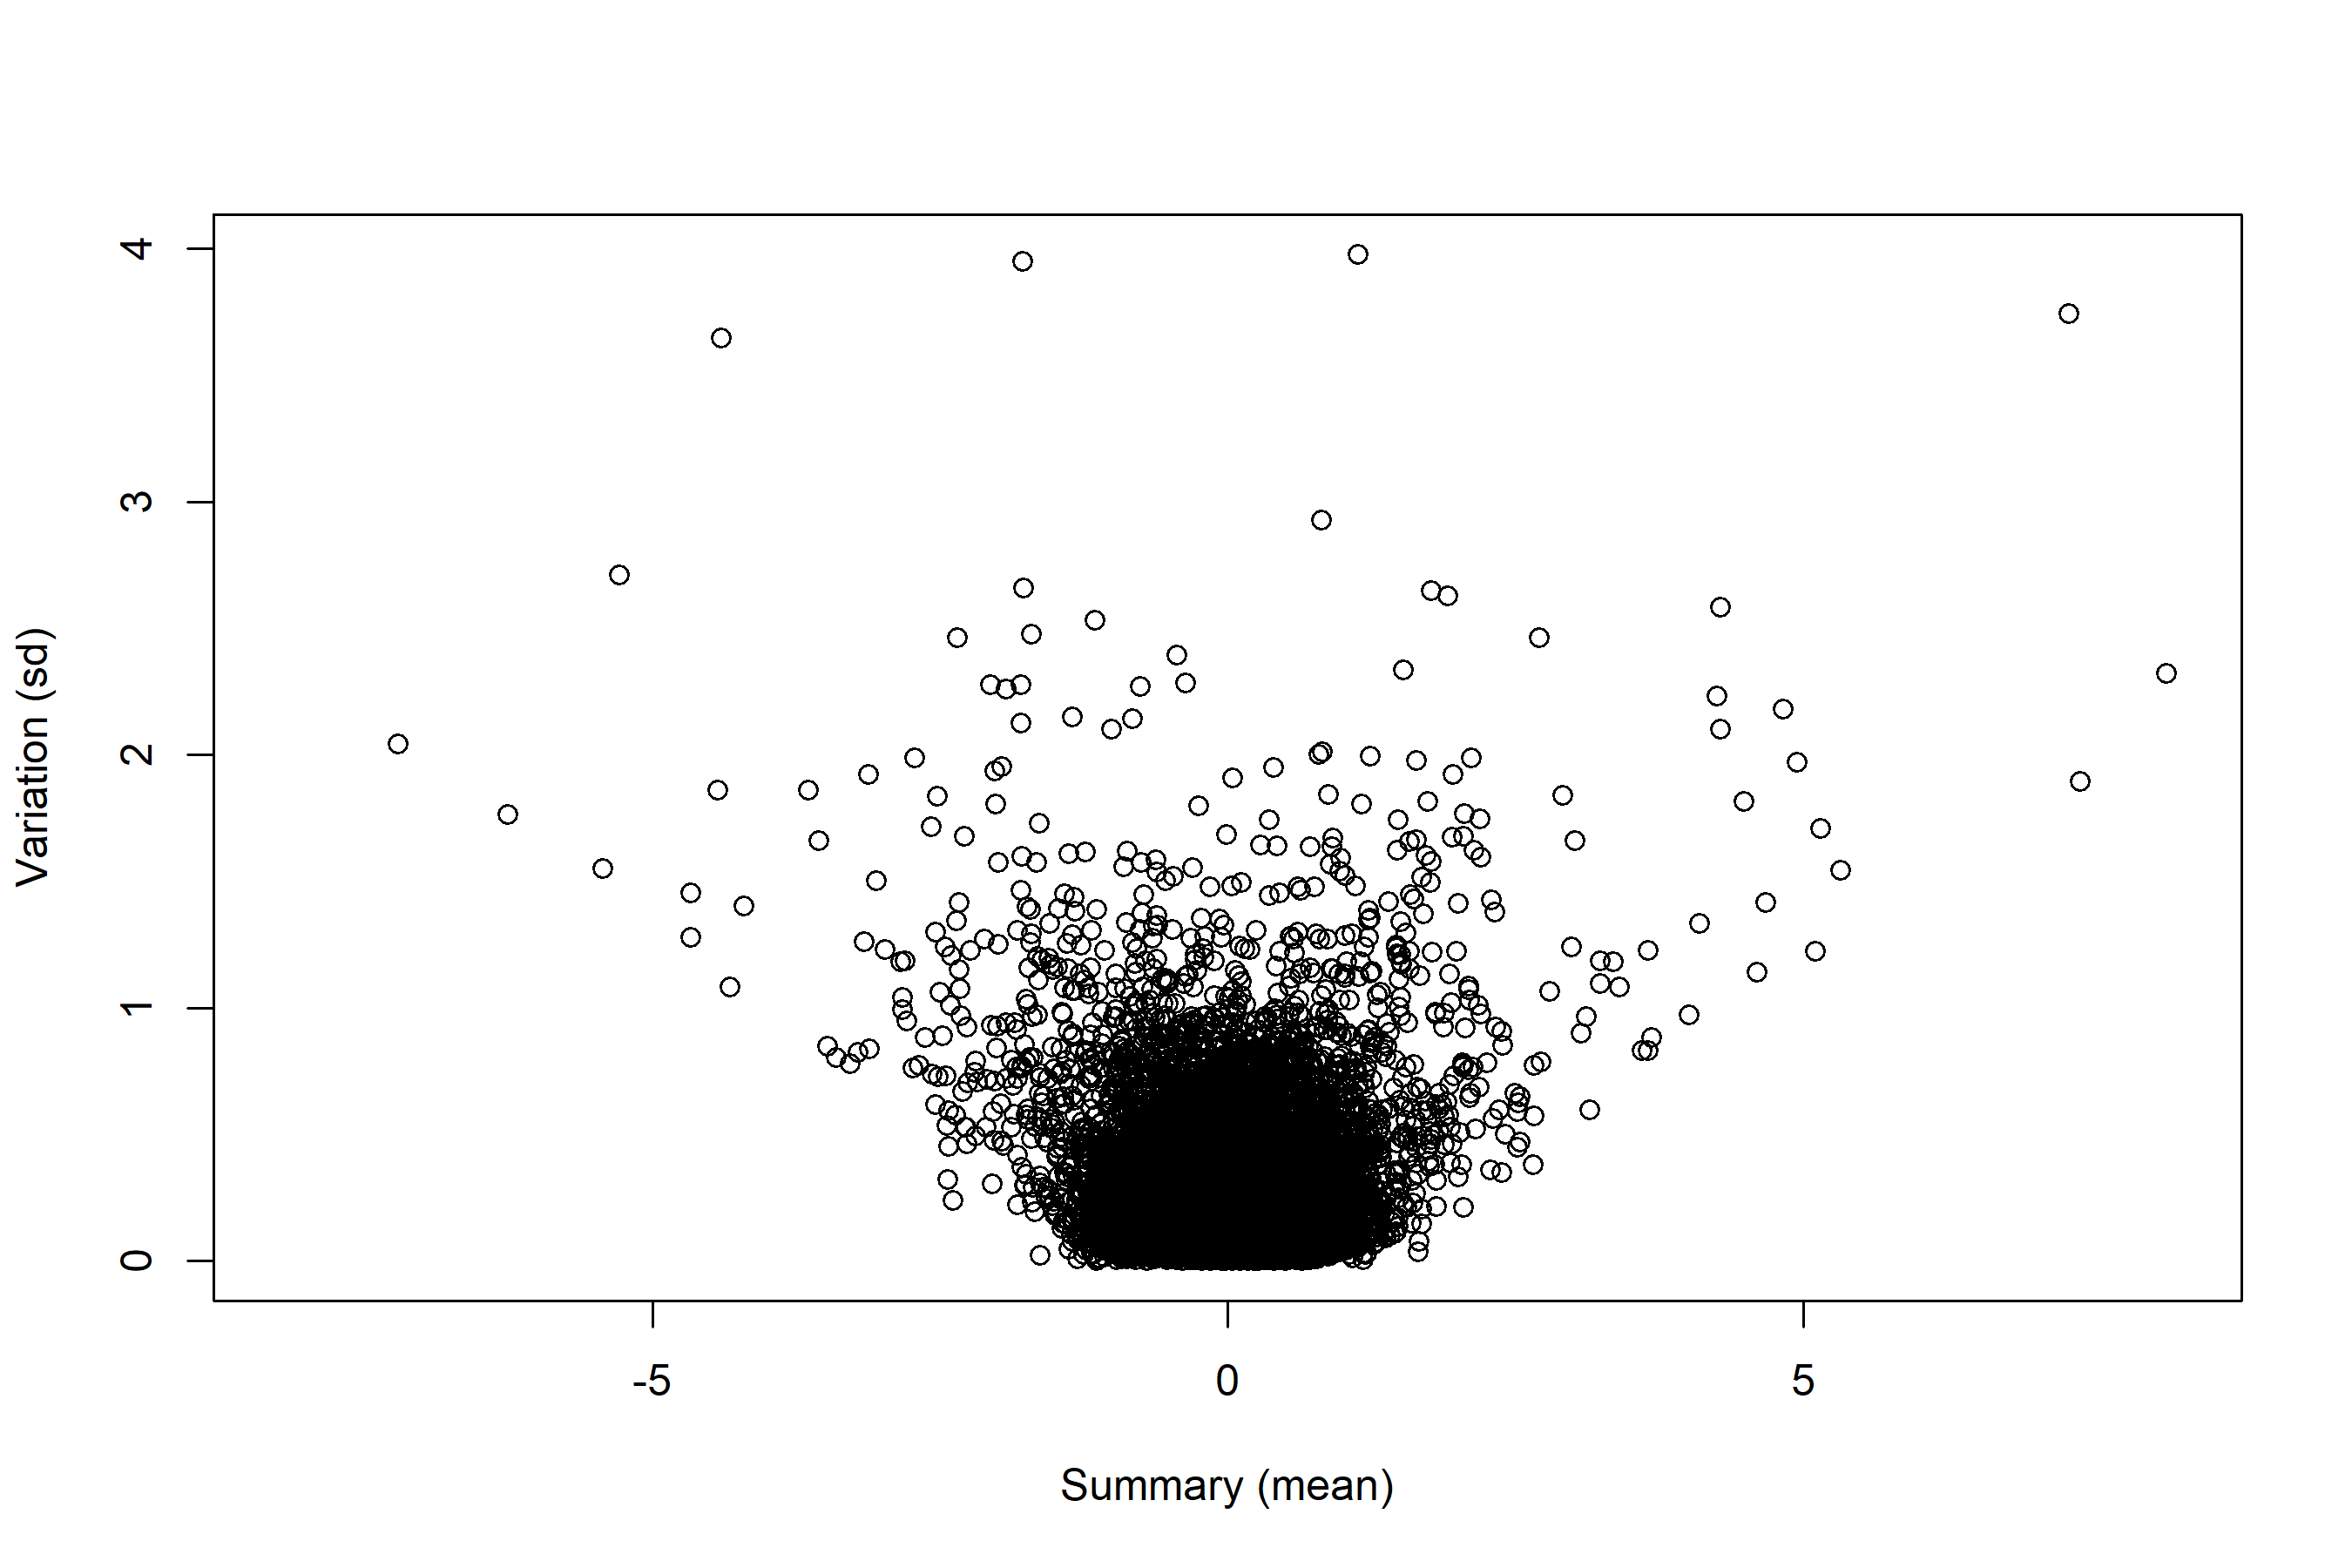
\includegraphics{README_files/figure-latex/unnamed-chunk-13-1.png}
\caption{SV-plot produced from a \texttt{GEVASummary} object using the
\texttt{geva.summarize} function with default parameters.}
\end{figure}

\hypertarget{delimitation-by-quantiles}{%
\subsection{Delimitation by quantiles}\label{delimitation-by-quantiles}}

After obtaining the \texttt{GEVASummary} object, the next step will be
calculating the quantiles for every SV-point. That can be done by
calling the \texttt{geva.quantiles} function as shown below:

\begin{Shaded}
\begin{Highlighting}[]
\CommentTok{# Calculates the quantiles from a GEVASummary object}
\NormalTok{gquants <-}\StringTok{ }\KeywordTok{geva.quantiles}\NormalTok{(gsummary)}
\end{Highlighting}
\end{Shaded}

The code above produces a \texttt{GEVAQuantiles} object which stores the
relevant partitions where the SV-points belong to. These partitions can
be viewed by calling \texttt{plot} on the produced object:

\begin{Shaded}
\begin{Highlighting}[]
\KeywordTok{plot}\NormalTok{(gquants)}
\end{Highlighting}
\end{Shaded}

\begin{figure}
\centering
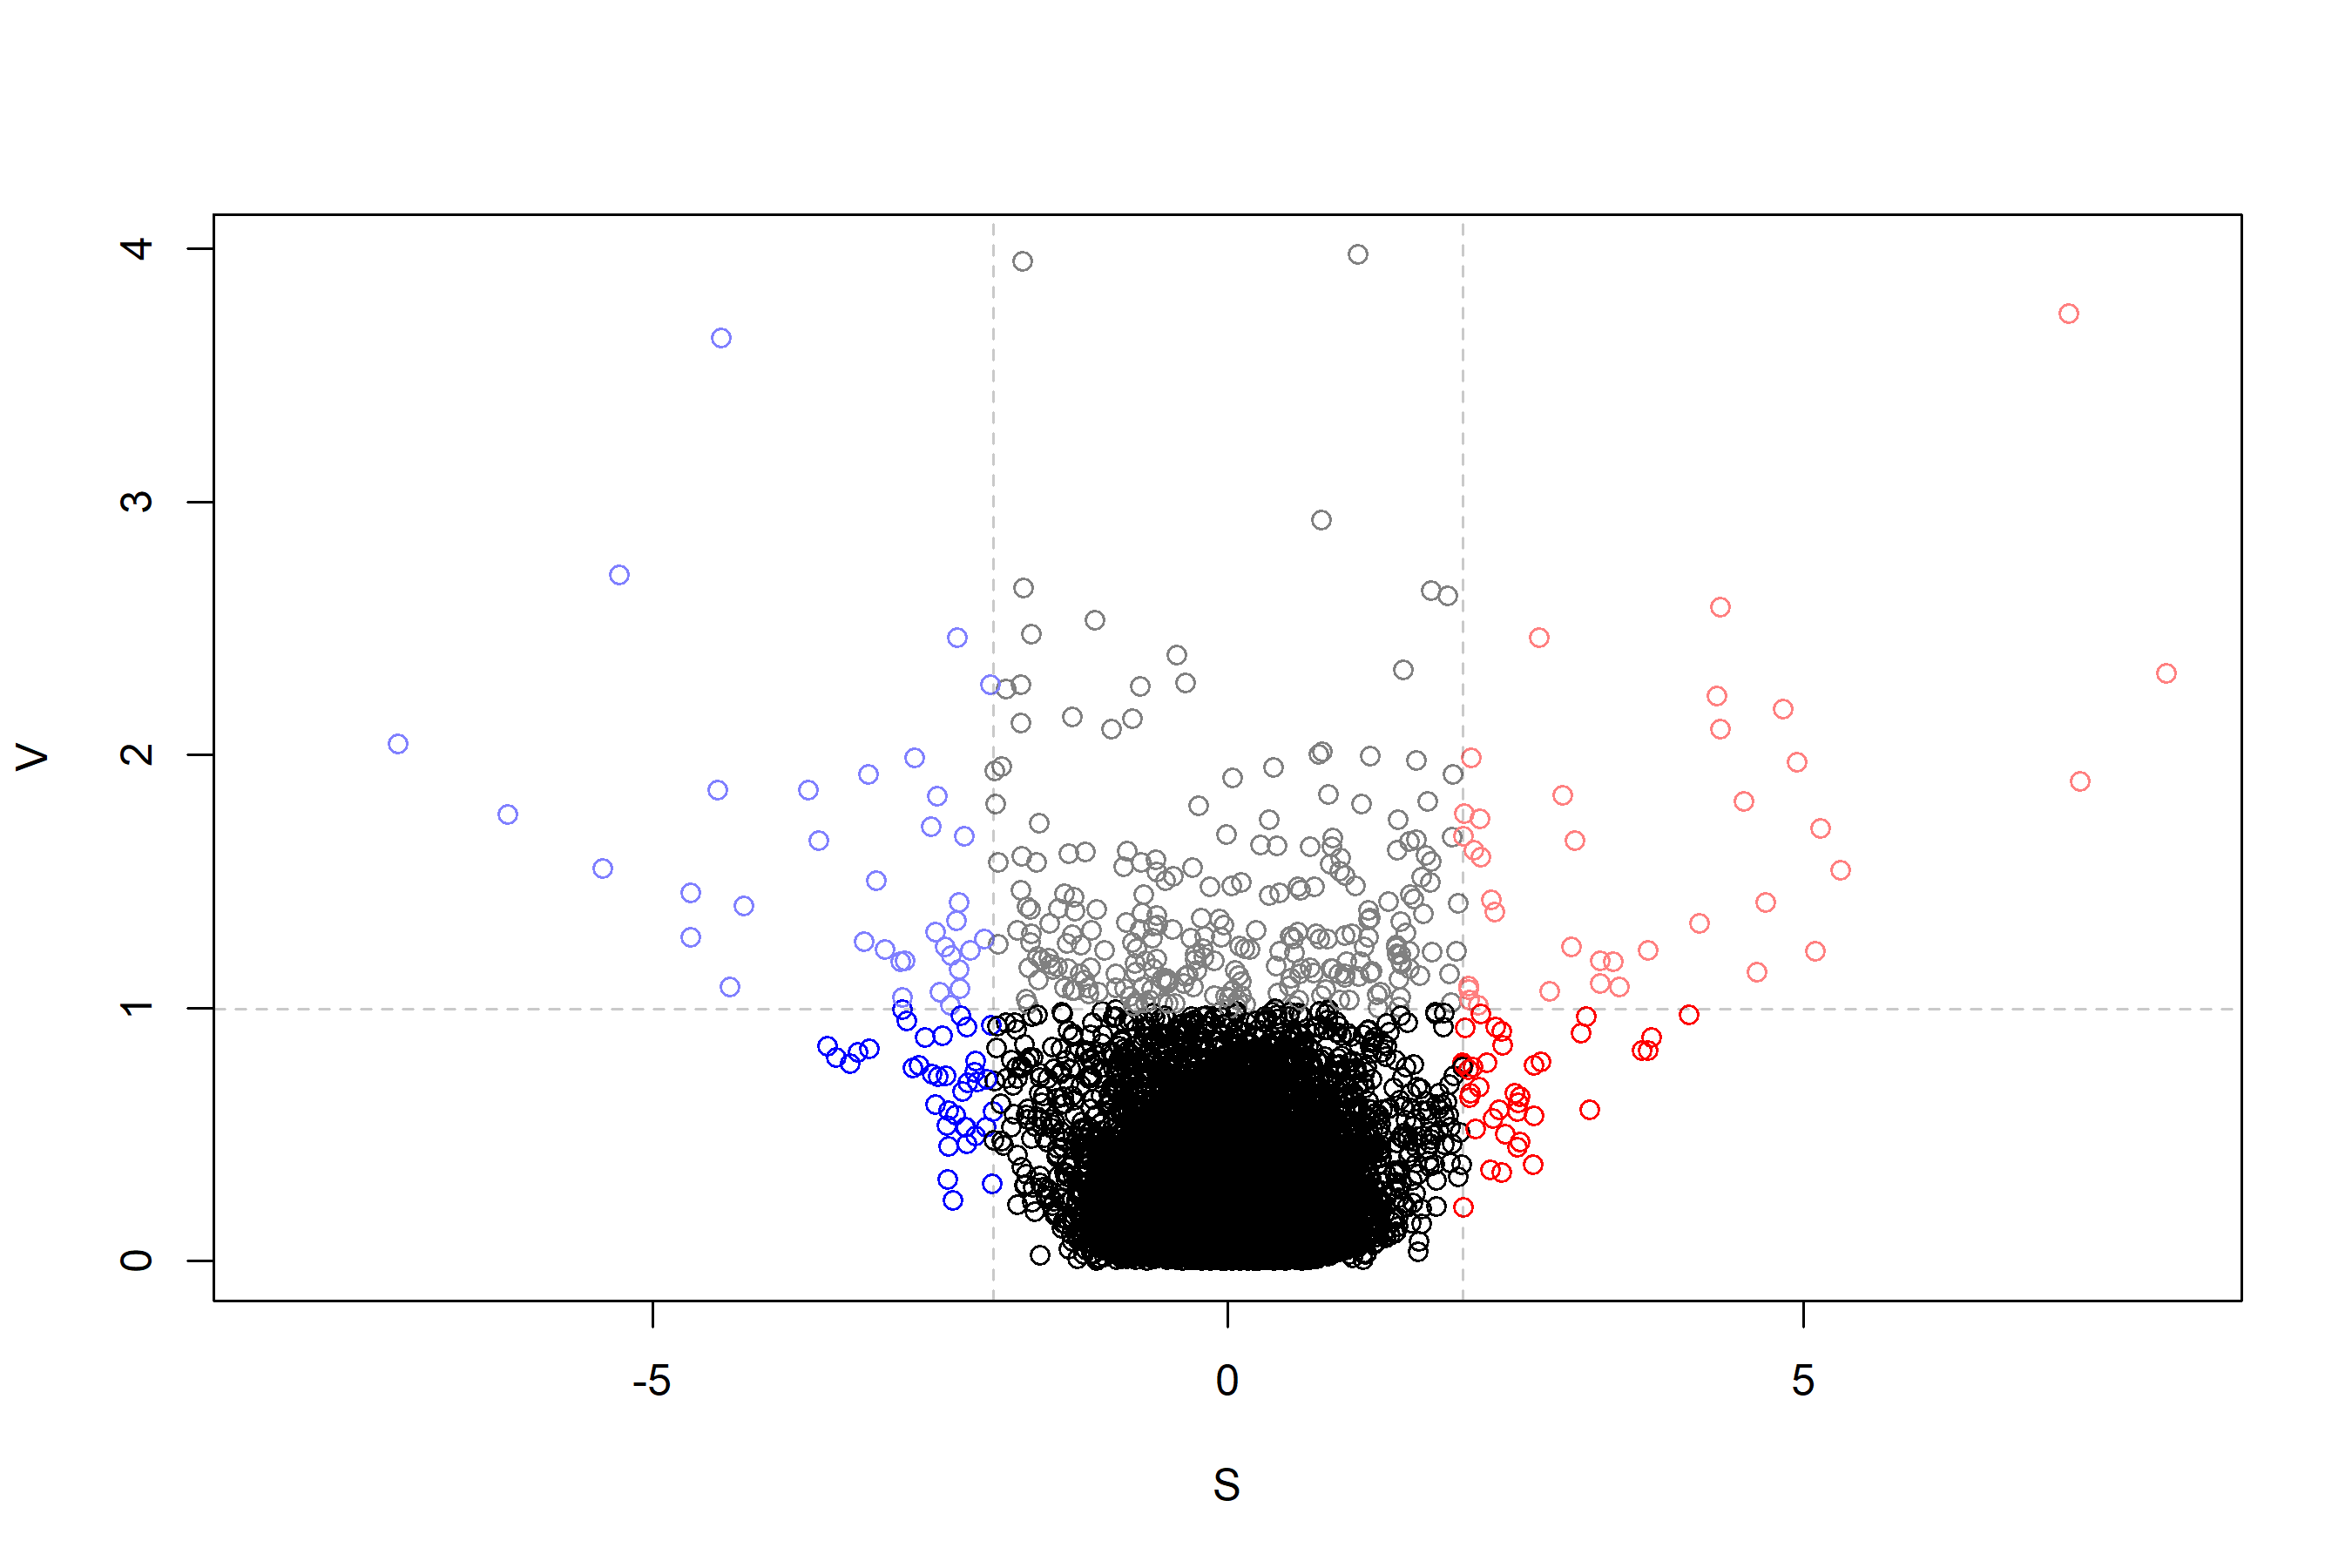
\includegraphics{README_files/figure-latex/unnamed-chunk-16-1.png}
\caption{SV-plot produced from a \texttt{GEVAQuantiles} object using the
\texttt{geva.quantiles} function with default parameters.}
\end{figure}

By default, the quantile detection is performed automatically using the
parameter \texttt{quantile.method="range.slice"} (for more methods, call
\texttt{?geva.quantiles}). However, the quantile delimiters can also be
specified in the \texttt{initial.thresholds} argument like the following
example:

\begin{Shaded}
\begin{Highlighting}[]
\CommentTok{# Calculates the quantiles from a GEVASummary object}
\CommentTok{# using custom delimiters}
\NormalTok{gquants <-}\StringTok{ }\KeywordTok{geva.quantiles}\NormalTok{(gsummary,}
                          \DataTypeTok{initial.thresholds =} \KeywordTok{c}\NormalTok{(}\DataTypeTok{S=}\DecValTok{1}\NormalTok{, }\DataTypeTok{V=}\FloatTok{0.5}\NormalTok{))}
\end{Highlighting}
\end{Shaded}

In this second example, thresholds of \texttt{1} and \texttt{0.5} were
defined for \texttt{S} and \texttt{V} axes. As it can be noted from the
SV-plot below, the results are purposely exaggerated and may not
represent a good separation between relevant points, but this option is
particularly useful to fine-tuning the quantile delimiters in situations
where the automatic methods did not present a satisfatory outcome.

\begin{figure}
\centering
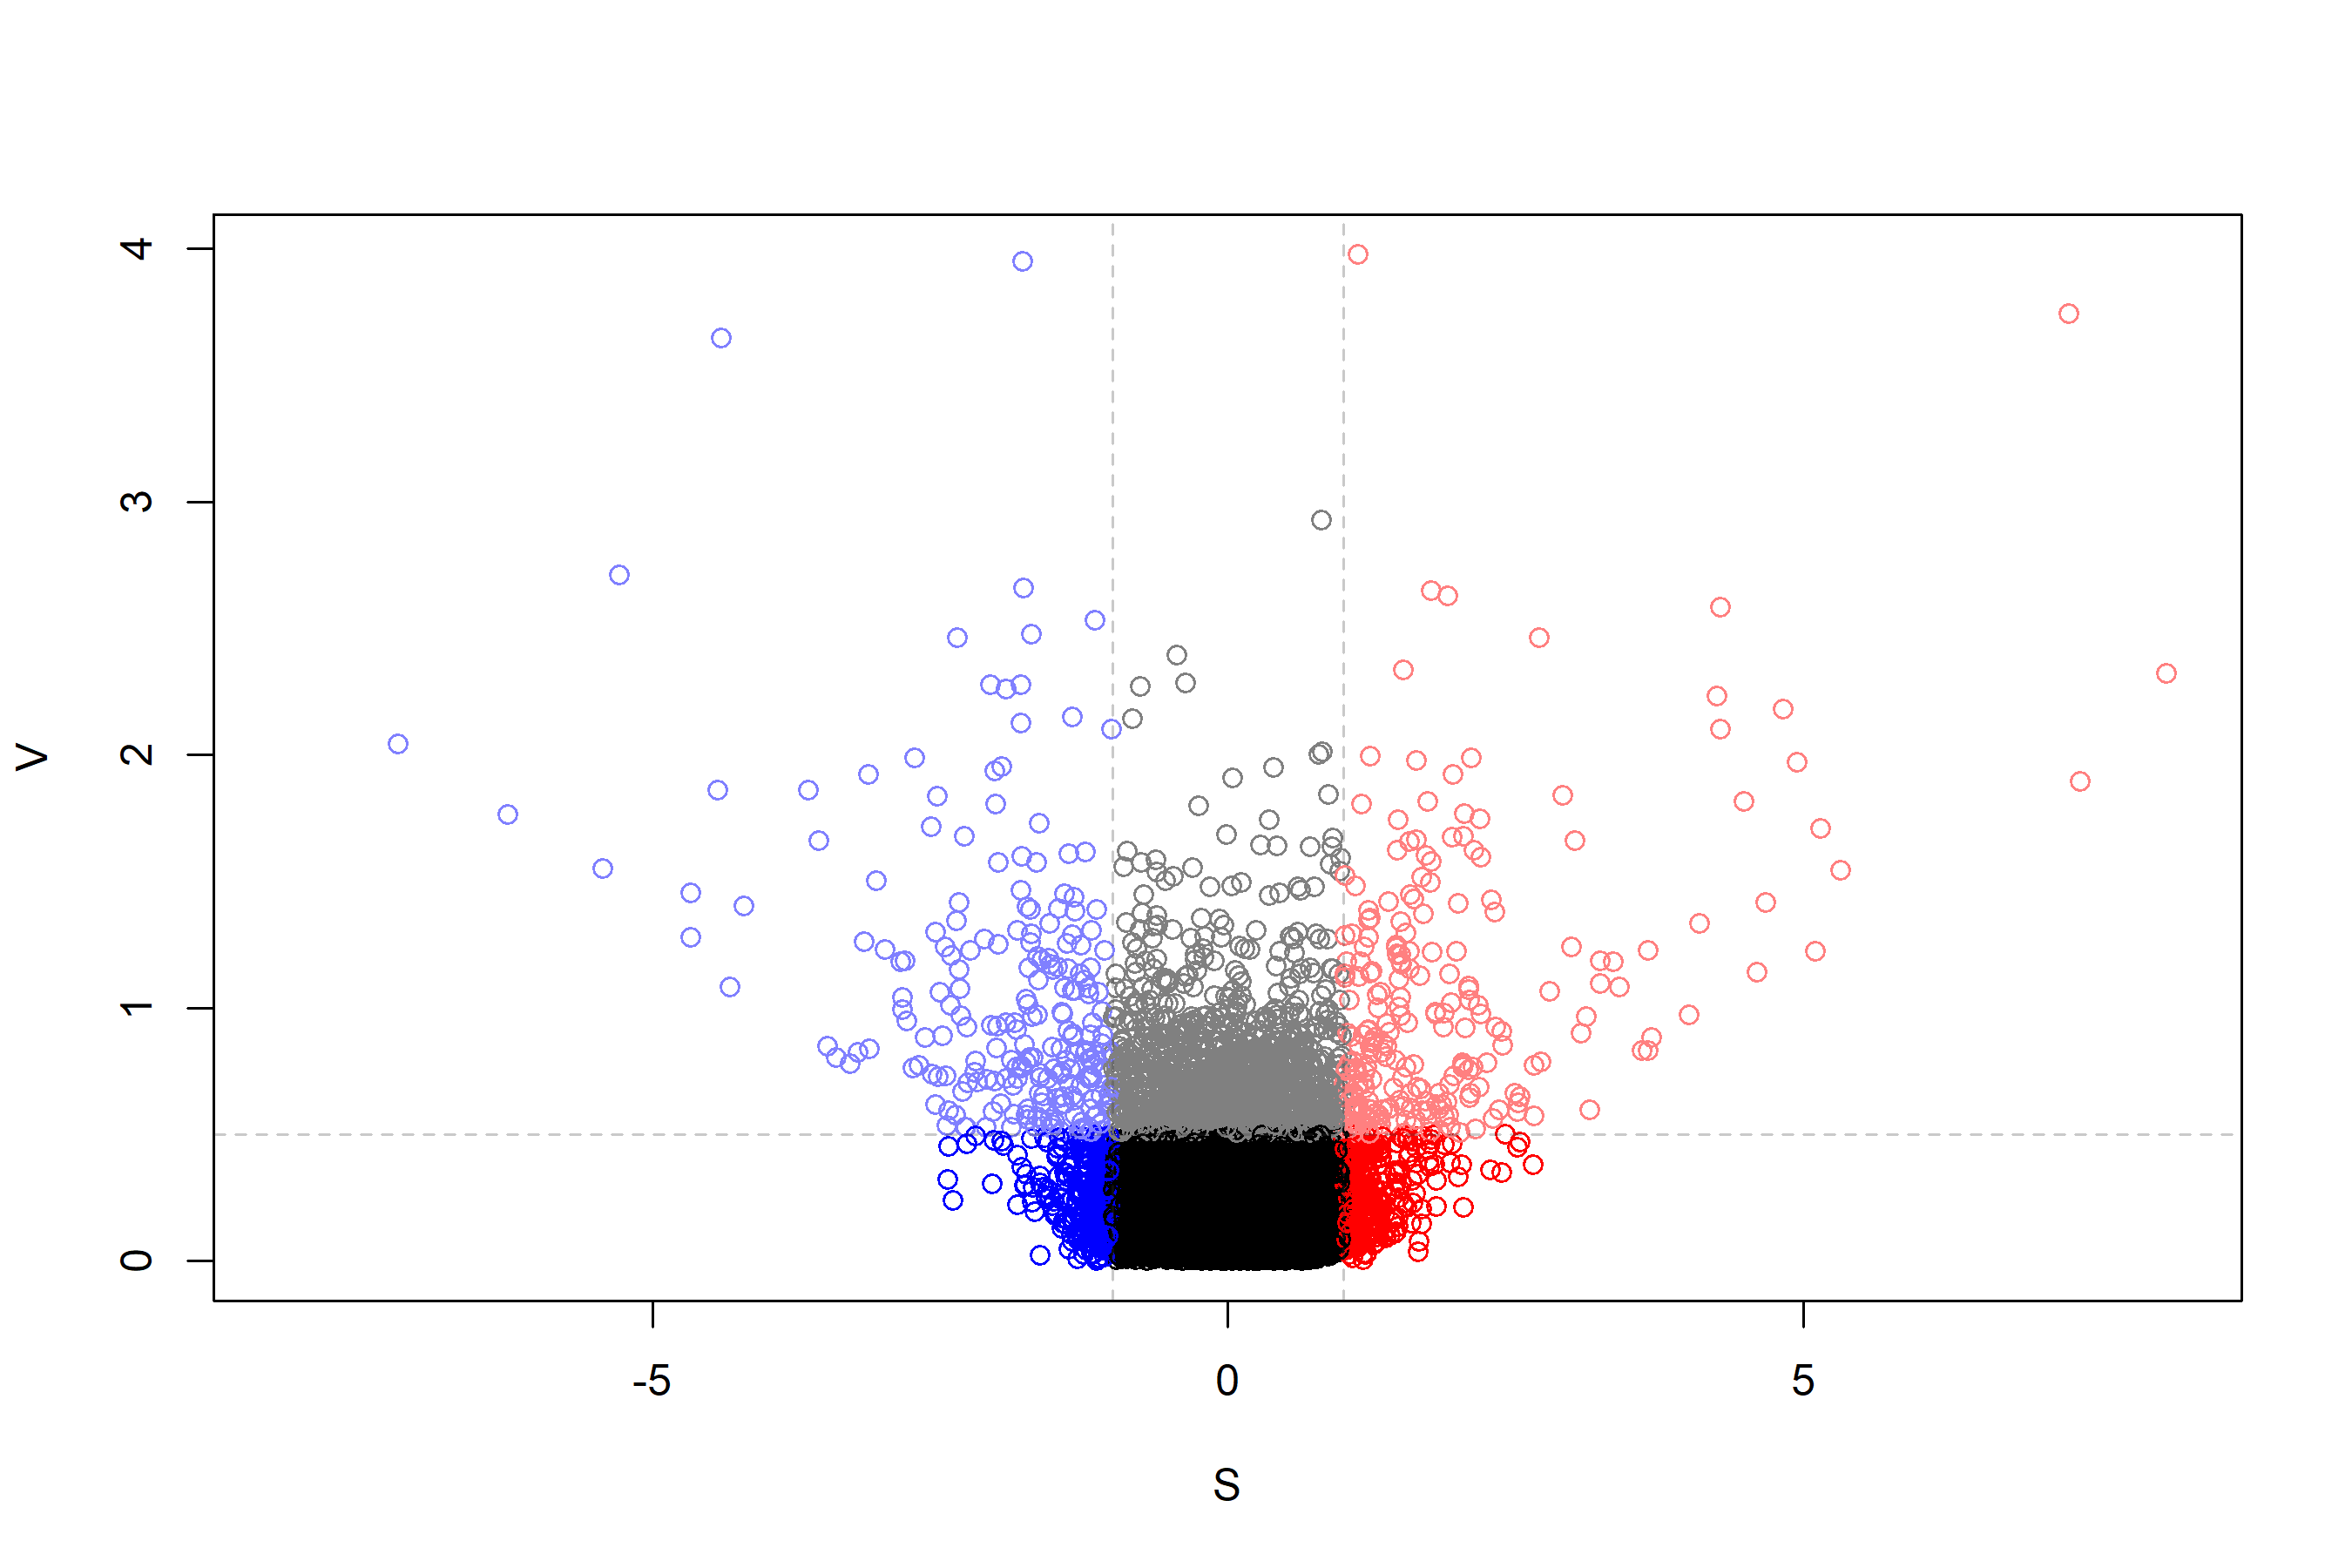
\includegraphics{README_files/figure-latex/unnamed-chunk-18-1.png}
\caption{SV-plot produced from a \texttt{GEVAQuantiles} object using the
\texttt{geva.quantiles} function using the
\texttt{initial.thresholds\ =\ c(S=1,\ V=0.5)} parameter.}
\end{figure}

Note that the quantile detection does not define an absolute cutoff, but
partitionizes the SV space into estimated regions containing qualitative
classifications for the SV points. These classifications may change
after combining the \texttt{GEVAQuantiles} with the results from the
next steps.

\hypertarget{clustering}{%
\subsection{Clustering}\label{clustering}}

In this step, a cluster analysis is applied to separate relevant points
from the agglomeration of non-differentially expressed genes. Such
agglomeration is mostly proeminent at the bottom-center region of a SV
plot and essentially portraits the least relevant portion of the
results.

\hypertarget{basic-usage-of-the-wrapper-function}{%
\subsubsection{Basic usage of the wrapper
function}\label{basic-usage-of-the-wrapper-function}}

The \texttt{geva.cluster} function is the top-level function for
clusters analysis and acts as a wrapper for more specific functions used
to group SV points. The inner function is specified by the
\texttt{cluster.method} argument with one of the following parameters:
(i) \texttt{"hierarchical"}, calls the \texttt{geva.hcluster} function
for hierarchical clustering; (ii) \texttt{"density"}, calls the
\texttt{geva.dcluster} function for density-based clustering; and (iii)
\texttt{"quantiles"}, calls the \texttt{geva.quantiles} function shown
in the previous section. Likewise, optional parameters from the top
funtion are passed to these calls.

In this section, only hierarchical and density-based clustering methods
are going to be discussed. Both methods use the \texttt{resolution}
argument, a single \texttt{numeric} between 0 and 1 that defines the
ratio of output clusters. If the \texttt{resolution} is \texttt{0.0}
(zero), the least number of clusters is assigned (\emph{i.e.}, usually
one or two), while if \texttt{1.0} then the maximum amount of clusters
is assigned (\emph{i.e.}, aproximately one cluster per point for
hierarchical clustering). For example, to apply \texttt{geva.cluster}
using hierarchical clustering at 30\% of the resolution, the function is
called as follows:

\begin{Shaded}
\begin{Highlighting}[]
\CommentTok{# Applies cluster analysis (30% resolution)}
\NormalTok{gcluster <-}\StringTok{ }\KeywordTok{geva.cluster}\NormalTok{(gsummary,}
                         \DataTypeTok{cluster.method=}\StringTok{"hierarchical"}\NormalTok{,}
                         \DataTypeTok{resolution=}\FloatTok{0.3}\NormalTok{)}
\end{Highlighting}
\end{Shaded}

The returned cluster data can be plotted using the generic \texttt{plot}
function:

\begin{Shaded}
\begin{Highlighting}[]
\KeywordTok{plot}\NormalTok{(gcluster)}
\end{Highlighting}
\end{Shaded}

\begin{figure}
\centering
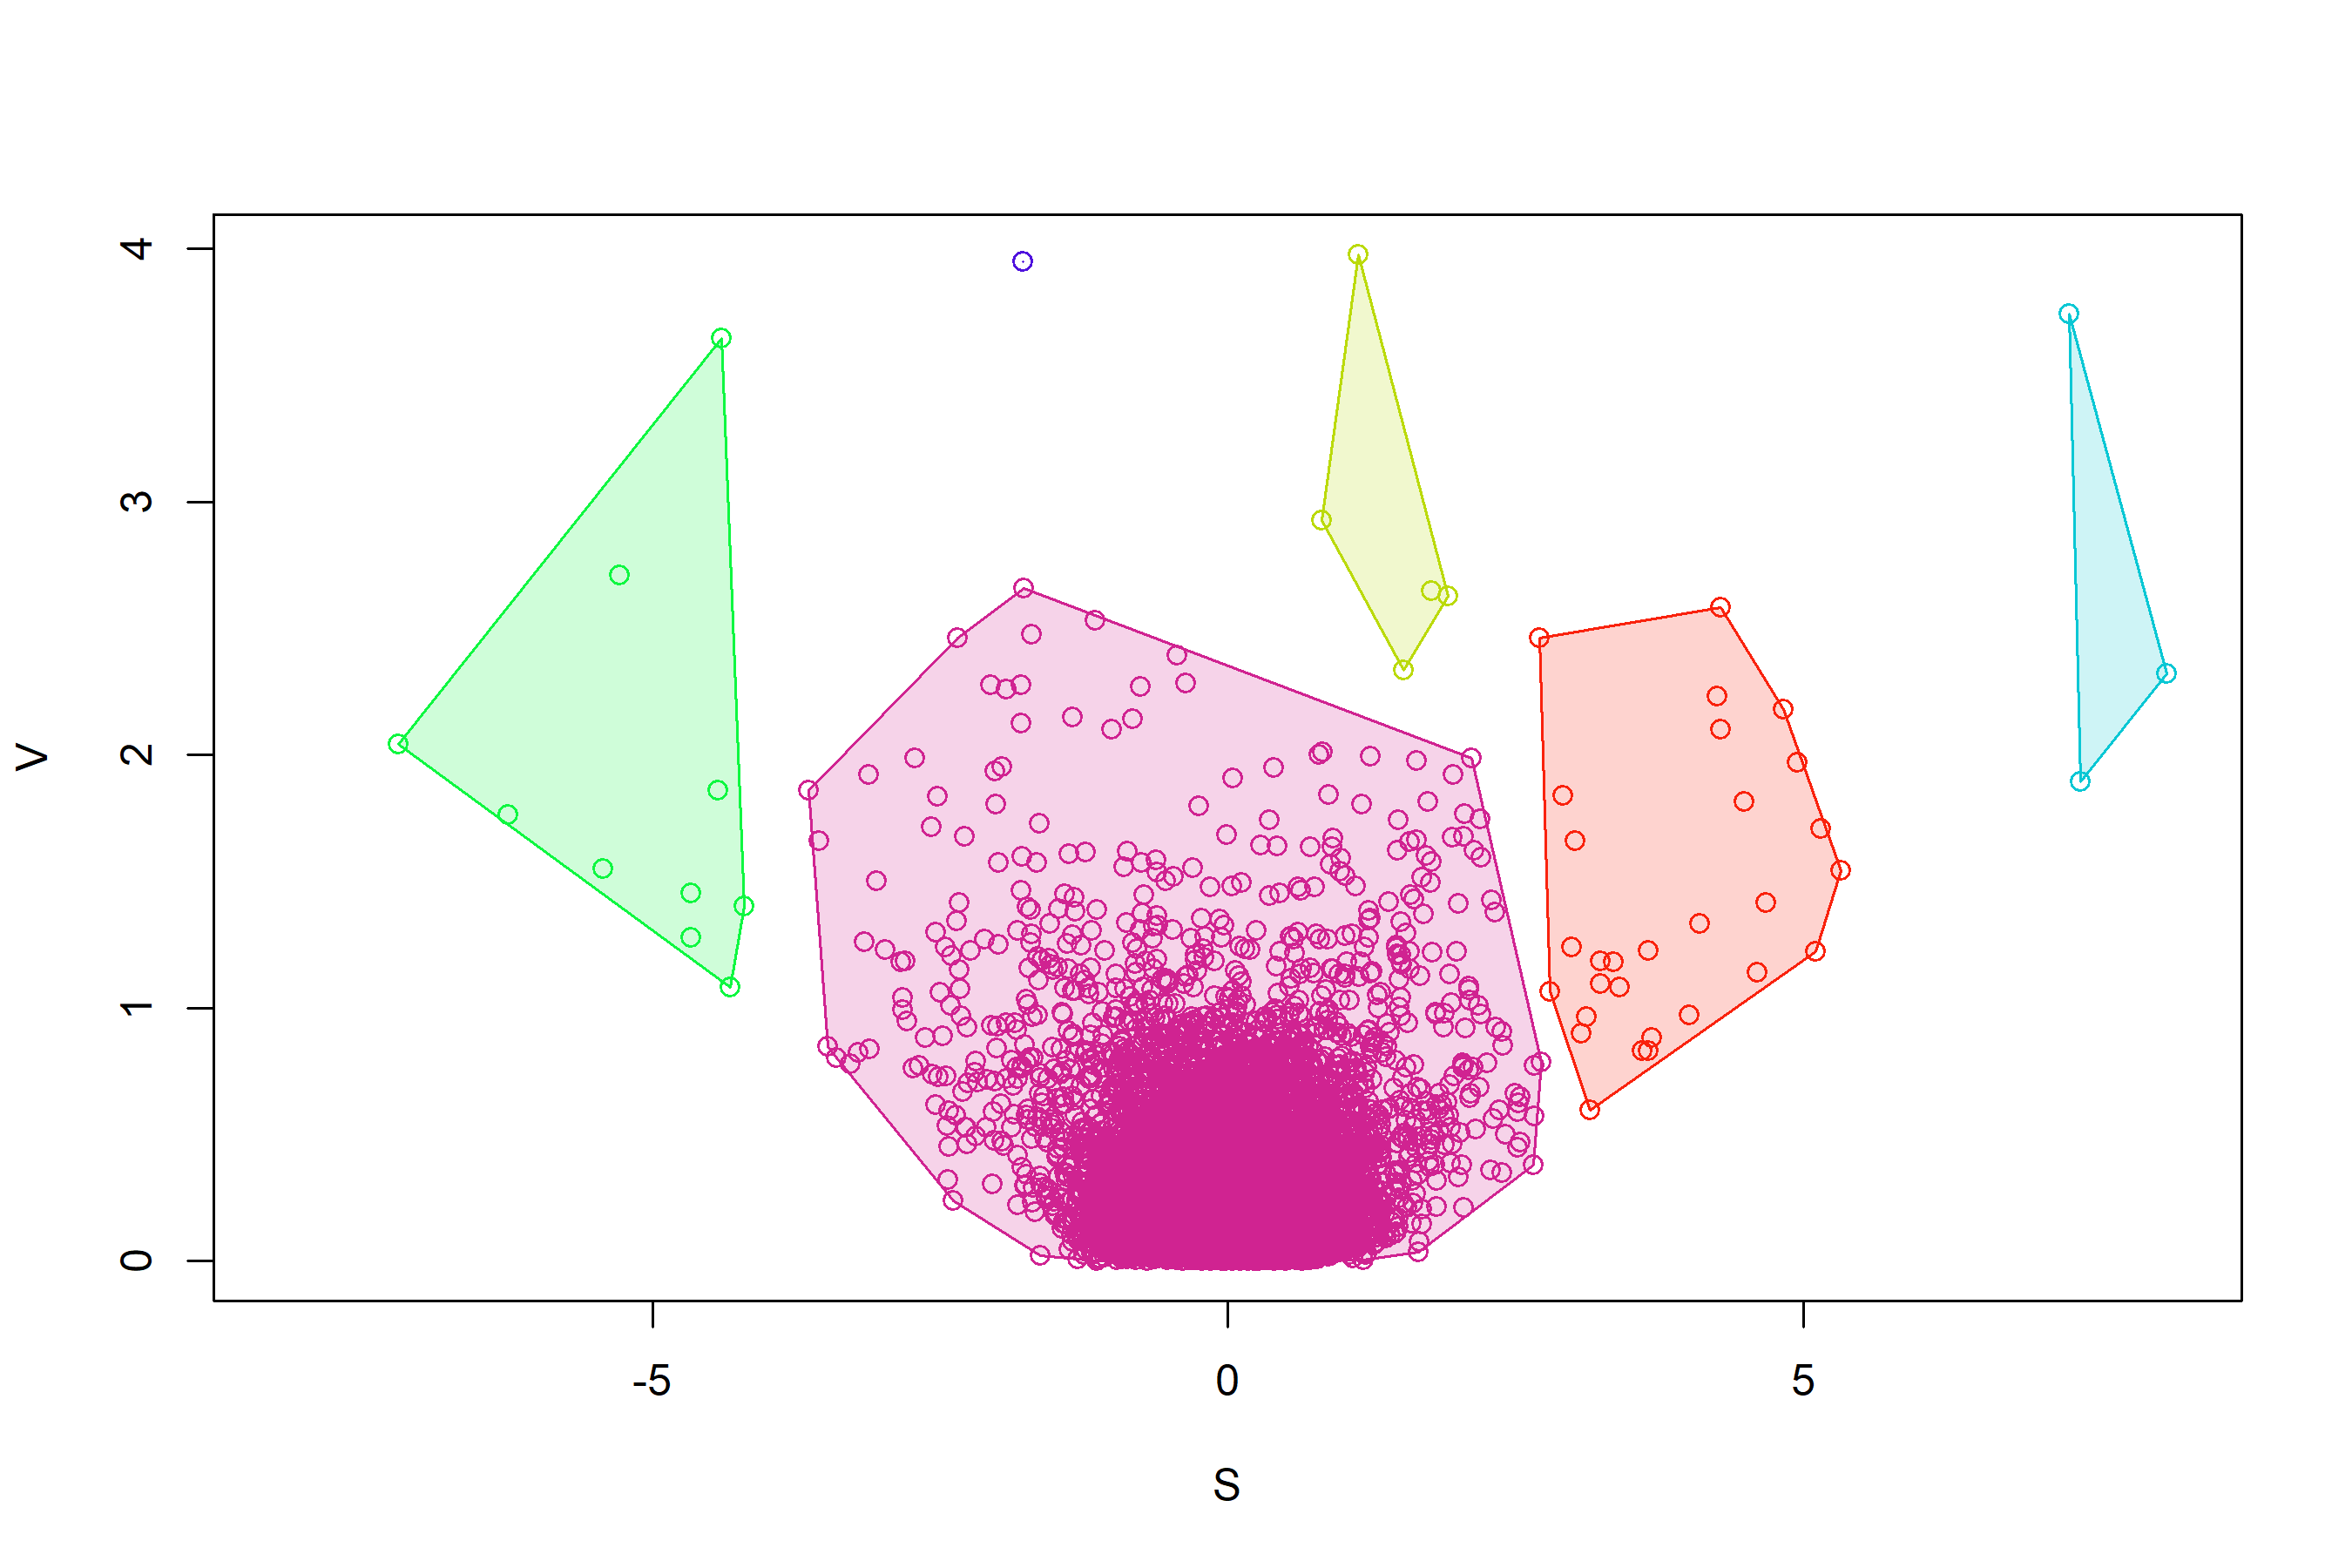
\includegraphics{README_files/figure-latex/unnamed-chunk-21-1.png}
\caption{SV-plot produced from a \texttt{GEVACluster} object using the
\texttt{geva.cluster} function with the hierarchical method and 30\% of
resolution.}
\end{figure}

\hypertarget{combining-clusters-with-summarized-data-optional}{%
\subsubsection{Combining clusters with summarized data
(Optional)}\label{combining-clusters-with-summarized-data-optional}}

Apart from its usage as a wrapper, the \texttt{geva.cluster} function
can also concatenate the summarized and grouped data into a single
object by setting \texttt{grouped.return=TRUE} in the arguments. With
this setup, the function will return a \texttt{GEVAGroupedSummary}
object, which is a \texttt{GEVASummary} that includes the list of group
sets (\texttt{GEVACluster} or \texttt{GEVAQuantile} objects). The code
below illustrates this specific use case:

\begin{Shaded}
\begin{Highlighting}[]
\CommentTok{# Applies cluster analysis with default parameters and}
\CommentTok{# returns a GEVAGroupedSummary}
\NormalTok{ggroupedsummary <-}\StringTok{ }\KeywordTok{geva.cluster}\NormalTok{(gsummary,}
                                \DataTypeTok{grouped.return =} \OtherTok{TRUE}\NormalTok{)}
\end{Highlighting}
\end{Shaded}

Alternatively, multiple group sets (clusters and quantiles) can be
combined directly to the summarized data by appending each of them with
\texttt{groupsets\textless{}-}, which also converts the
\texttt{GEVASummary} to a \texttt{GEVAGroupedSummary} object. For
example, assuming that \texttt{gquants} and \texttt{gcluster} are output
values from the previous quantiles (\texttt{geva.quantiles}) and
clustering (\texttt{geva.cluster}) steps, respectively, the code would
be:

\begin{Shaded}
\begin{Highlighting}[]
\CommentTok{# Makes a safe copy of the summary data}
\NormalTok{ggroupedsummary <-}\StringTok{ }\NormalTok{gsummary}
\CommentTok{# Appends the quantiles data}
\KeywordTok{groupsets}\NormalTok{(ggroupedsummary) <-}\StringTok{ }\NormalTok{gquants}
\CommentTok{# Appends the clustered data}
\KeywordTok{groupsets}\NormalTok{(ggroupedsummary) <-}\StringTok{ }\NormalTok{gcluster}

\CommentTok{# Draws a SV plot with grouped highlights (optional)}
\KeywordTok{plot}\NormalTok{(ggroupedsummary)}
\end{Highlighting}
\end{Shaded}

\begin{figure}
\centering
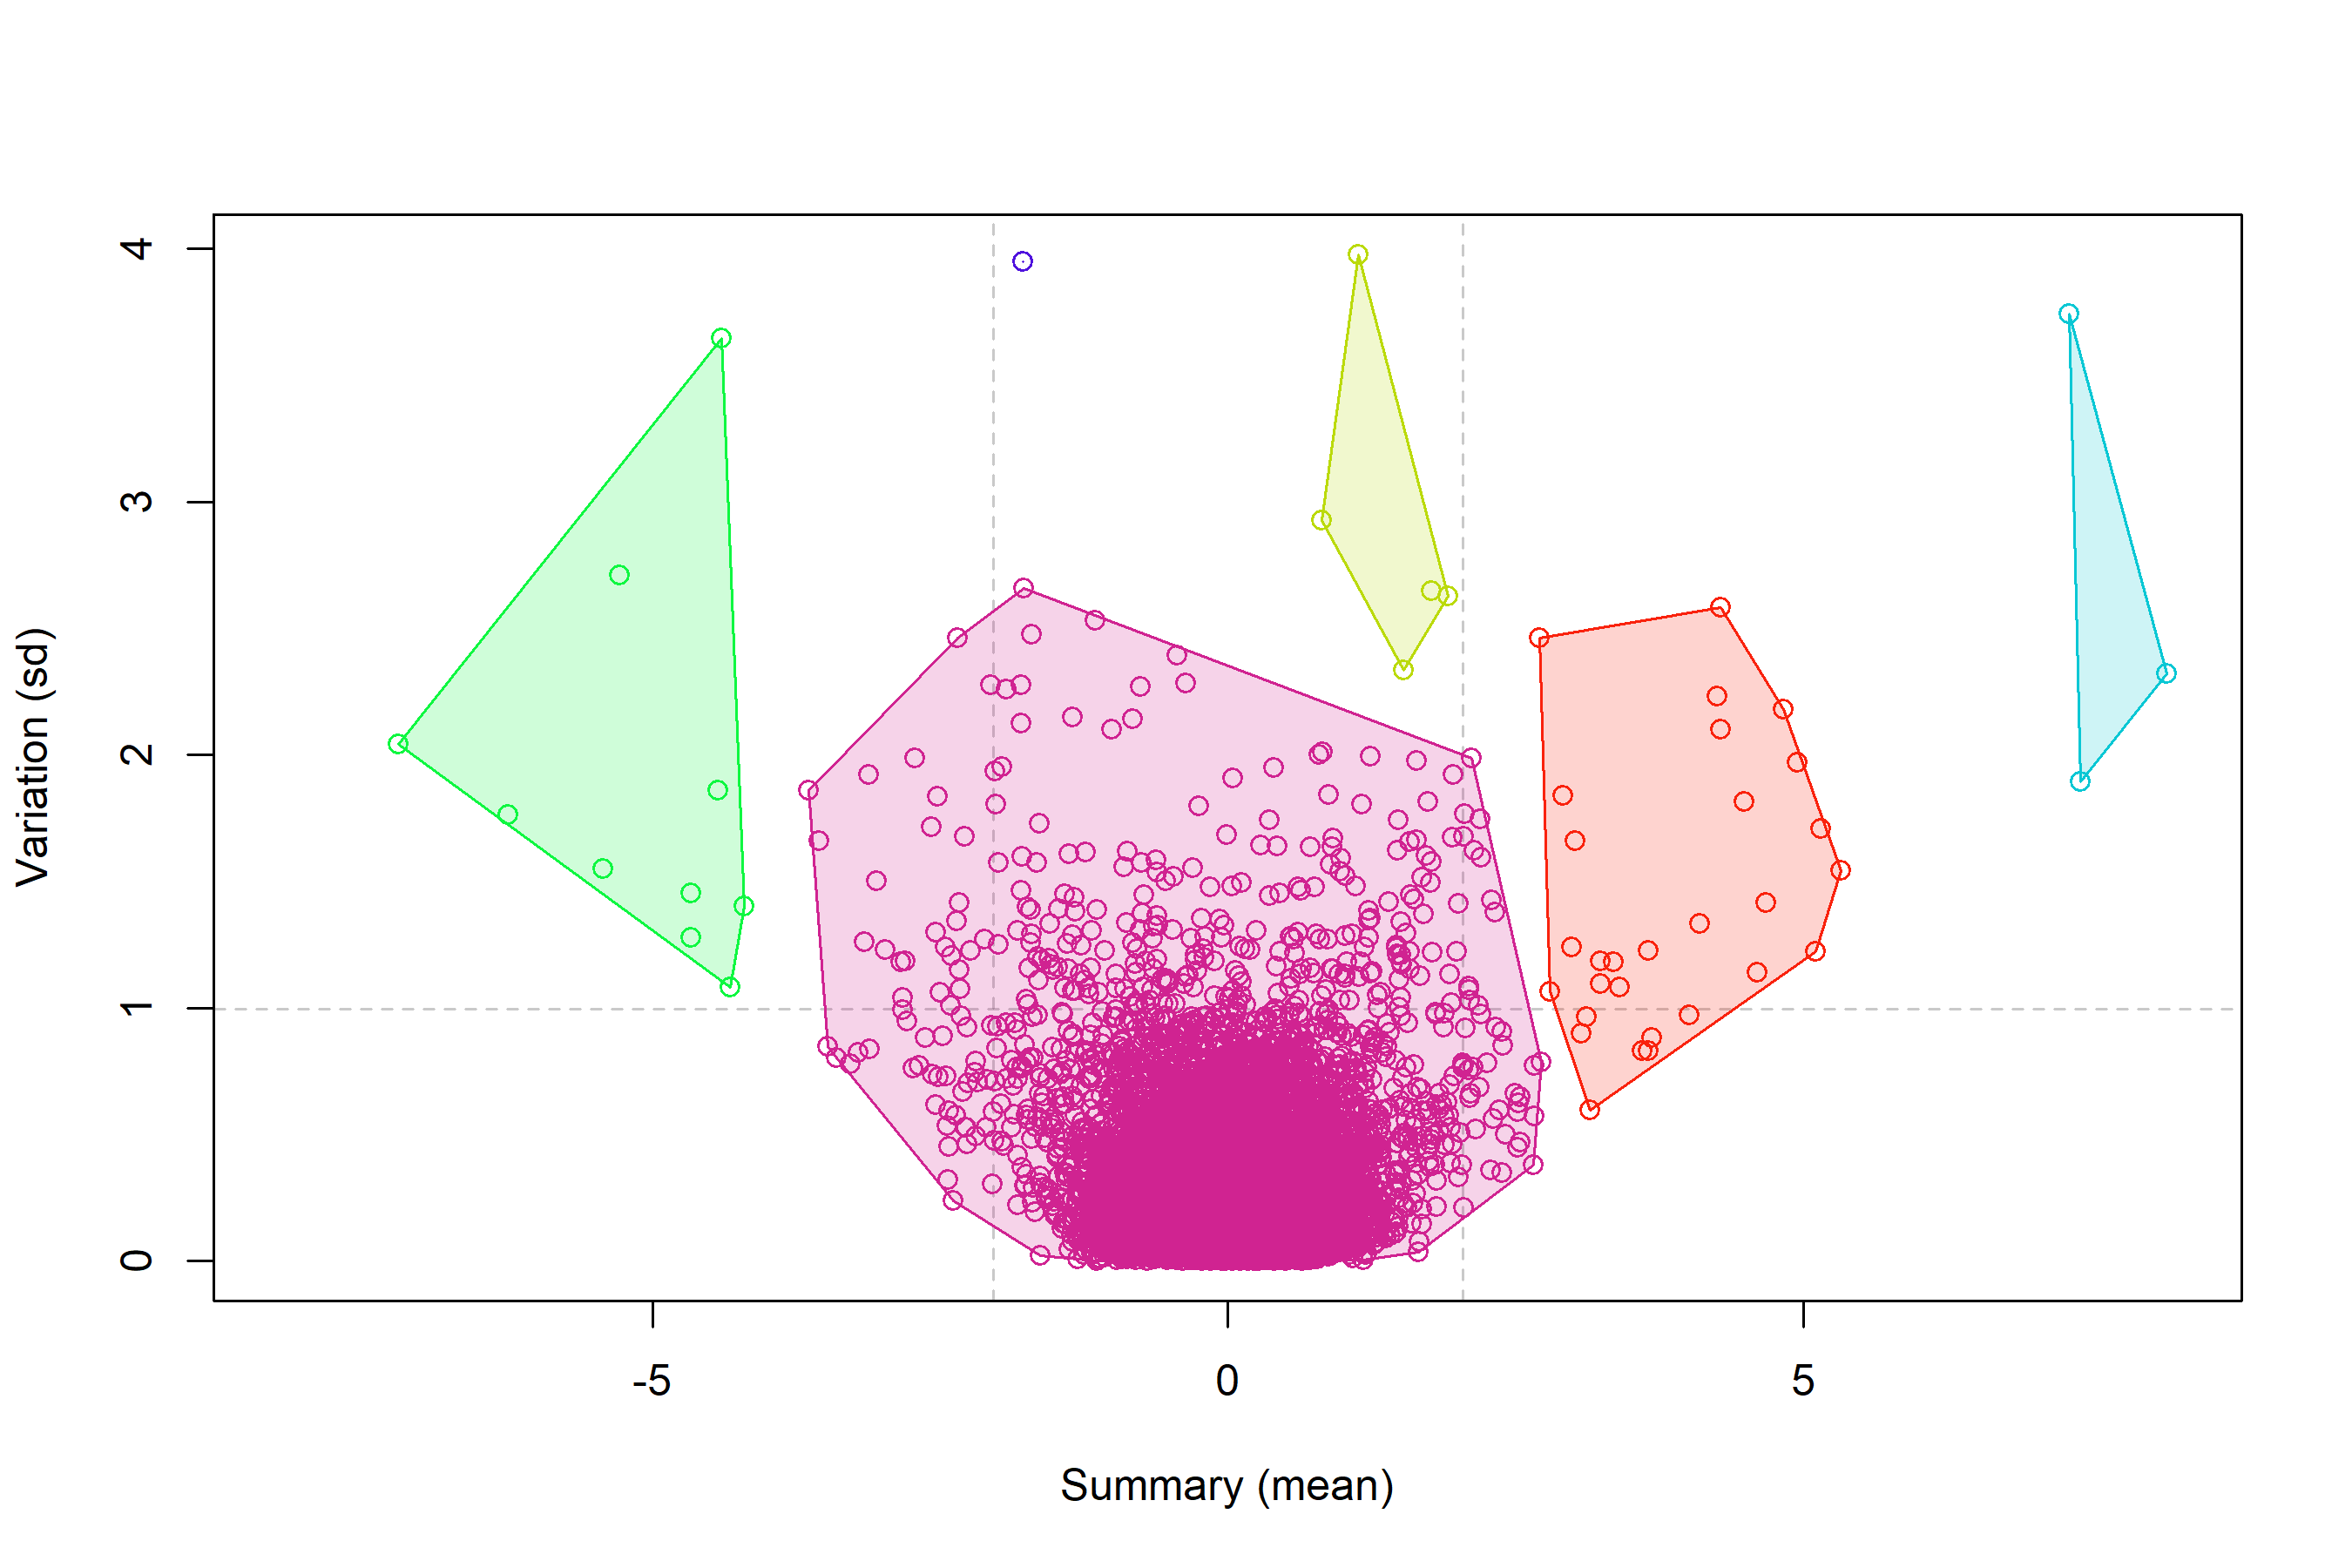
\includegraphics{README_files/figure-latex/unnamed-chunk-24-1.png}
\caption{SV-plot produced from a \texttt{GEVAGroupedSummary} object
after appending the \texttt{GEVAQuantiles} and \texttt{GEVACluster}
objects from previous steps.}
\end{figure}

\clearpage

\hypertarget{attaining-and-accessing-the-results}{%
\section{Attaining and accessing the
results}\label{attaining-and-accessing-the-results}}

After obtaining the quantiles and clusters from the summarized data in
the previous step, now the entire data can be taken together to prospect
the final classifications for each gene. This section presents the final
steps to obtain the results table and some basic method to access it.

\hypertarget{final-concatenation-and-factor-analysis}{%
\subsection{Final concatenation and factor
analysis}\label{final-concatenation-and-factor-analysis}}

In this final analysis step, the \texttt{geva.finalize} function takes a
\texttt{GEVASummary} object as argument in addition to the other values
returned from the intermediate steps, including the
\texttt{GEVAQuantiles} and \texttt{GEVACluster} objects. Alternatively,
a \texttt{GEVAGroupedSummary} object containing these intermediate
results can be provided alone. The function will correct the quantiles
based on the clustered points and return a classification that fits
better both group assignments. Furthermore, if factors (groups of
experimental conditions) were defined for the input columns,
\texttt{geva.finalize} will also look for DE variations according to
these factors, thereby unlocking two additional possible classifications
(\texttt{"factor-dependent"} and \texttt{"factor-specific"}). The
possible use cases are discussed in the following sub-sections:

\hypertarget{alternative-1-without-factors}{%
\subsubsection{Alternative 1 -- Without
factors}\label{alternative-1-without-factors}}

If factors were not included, no additional steps are required. The
function call is done by passing the \texttt{GEVASummary},
\texttt{GEVAQuantiles} and \texttt{GEVACluster} from previous steps:

\begin{Shaded}
\begin{Highlighting}[]
\CommentTok{# Calculates the final classifications based on the}
\CommentTok{# intermediate results from previous steps}
\NormalTok{gresults <-}\StringTok{ }\KeywordTok{geva.finalize}\NormalTok{(gsummary, gquants, gcluster)}
\end{Highlighting}
\end{Shaded}

Or, if a \texttt{GEVAGroupedSummary} object is provided:

\begin{Shaded}
\begin{Highlighting}[]
\CommentTok{# Calculates the final classifications based on the}
\CommentTok{# intermediate results from previous steps}
\NormalTok{gresults <-}\StringTok{ }\KeywordTok{geva.finalize}\NormalTok{(ggroupedsummary)}
\end{Highlighting}
\end{Shaded}

Note that, without factors, the only relevant classification is
\texttt{"similar"} (\emph{i.e.}, genes with similar \emph{logFC} values
among all experiments).

\hypertarget{alternative-2-with-factors}{%
\subsubsection{Alternative 2 -- With
factors}\label{alternative-2-with-factors}}

Factors can be accessed and assigned to a \texttt{GEVAInput} object
using \texttt{factors} and \texttt{factors\textless{}-}, respectively,
and both accessors are valid for \texttt{GEVASummary} as well. The
factors being set must be a \texttt{factor} or \texttt{character} vector
whose length is equivalent to the number of columns, and it must contain
at least two values per level to be considered since the factor analysis
is based on ANOVA.

For instance, considering a \texttt{GEVASummary} object that stores a
\texttt{GEVAInput} with 6 columns (experimental results), if one wants
to separate these columns into 3 factors (`g1', `g2', and `g3'), the
following code could be applied:

\begin{Shaded}
\begin{Highlighting}[]
\CommentTok{# Assigning factors to an example input with 6 columns}

\CommentTok{# Example with GEVAInput}
\KeywordTok{factors}\NormalTok{(ginput) <-}\StringTok{ }\KeywordTok{c}\NormalTok{(}\StringTok{'g1'}\NormalTok{, }\StringTok{'g1'}\NormalTok{, }\StringTok{'g2'}\NormalTok{, }\StringTok{'g2'}\NormalTok{, }\StringTok{'g3'}\NormalTok{, }\StringTok{'g3'}\NormalTok{)}

\CommentTok{# Example with GEVAInput (using factor class)}
\KeywordTok{factors}\NormalTok{(ginput) <-}\StringTok{ }\KeywordTok{factor}\NormalTok{(}\KeywordTok{c}\NormalTok{(}\StringTok{'g1'}\NormalTok{, }\StringTok{'g1'}\NormalTok{, }\StringTok{'g2'}\NormalTok{,}
                            \StringTok{'g2'}\NormalTok{, }\StringTok{'g3'}\NormalTok{, }\StringTok{'g3'}\NormalTok{))}

\CommentTok{# Example with GEVASummary}
\KeywordTok{factors}\NormalTok{(gsummary) <-}\StringTok{ }\KeywordTok{c}\NormalTok{(}\StringTok{'g1'}\NormalTok{, }\StringTok{'g1'}\NormalTok{, }\StringTok{'g2'}\NormalTok{, }\StringTok{'g2'}\NormalTok{, }\StringTok{'g3'}\NormalTok{, }\StringTok{'g3'}\NormalTok{)}
\end{Highlighting}
\end{Shaded}

By including factors in the current analysis, some optional arguments
related to the factor analysis become available in
\texttt{geva.finalize}. The \texttt{p.value}, for instance, determines
the significance cutoff employed in ANOVA tests (by default, this value
is \texttt{0.05} for \(\alpha < 0.05\)). In this case, the function call
becomes:

\begin{Shaded}
\begin{Highlighting}[]
\CommentTok{# Calculates the final classifications based on the}
\CommentTok{# intermediate results from previous steps}
\NormalTok{gresults <-}\StringTok{ }\KeywordTok{geva.finalize}\NormalTok{(gsummary, gquants, gcluster,}
                          \DataTypeTok{p.value=}\FloatTok{0.05}\NormalTok{)}
\end{Highlighting}
\end{Shaded}

Or, if a \texttt{GEVAGroupedSummary} object is provided:

\begin{Shaded}
\begin{Highlighting}[]
\CommentTok{# Calculates the final classifications based on the}
\CommentTok{# intermediate results from previous steps}
\NormalTok{gresults <-}\StringTok{ }\KeywordTok{geva.finalize}\NormalTok{(ggroupedsummary, }\DataTypeTok{p.value=}\FloatTok{0.05}\NormalTok{)}
\end{Highlighting}
\end{Shaded}

The results can be plotted into a SV plot similarly as in the previous
steps, but now only the relevant points will be colored while the rest
are painted in black or gray:

\begin{Shaded}
\begin{Highlighting}[]
\KeywordTok{plot}\NormalTok{(gresults)}
\end{Highlighting}
\end{Shaded}

\begin{figure}
\centering
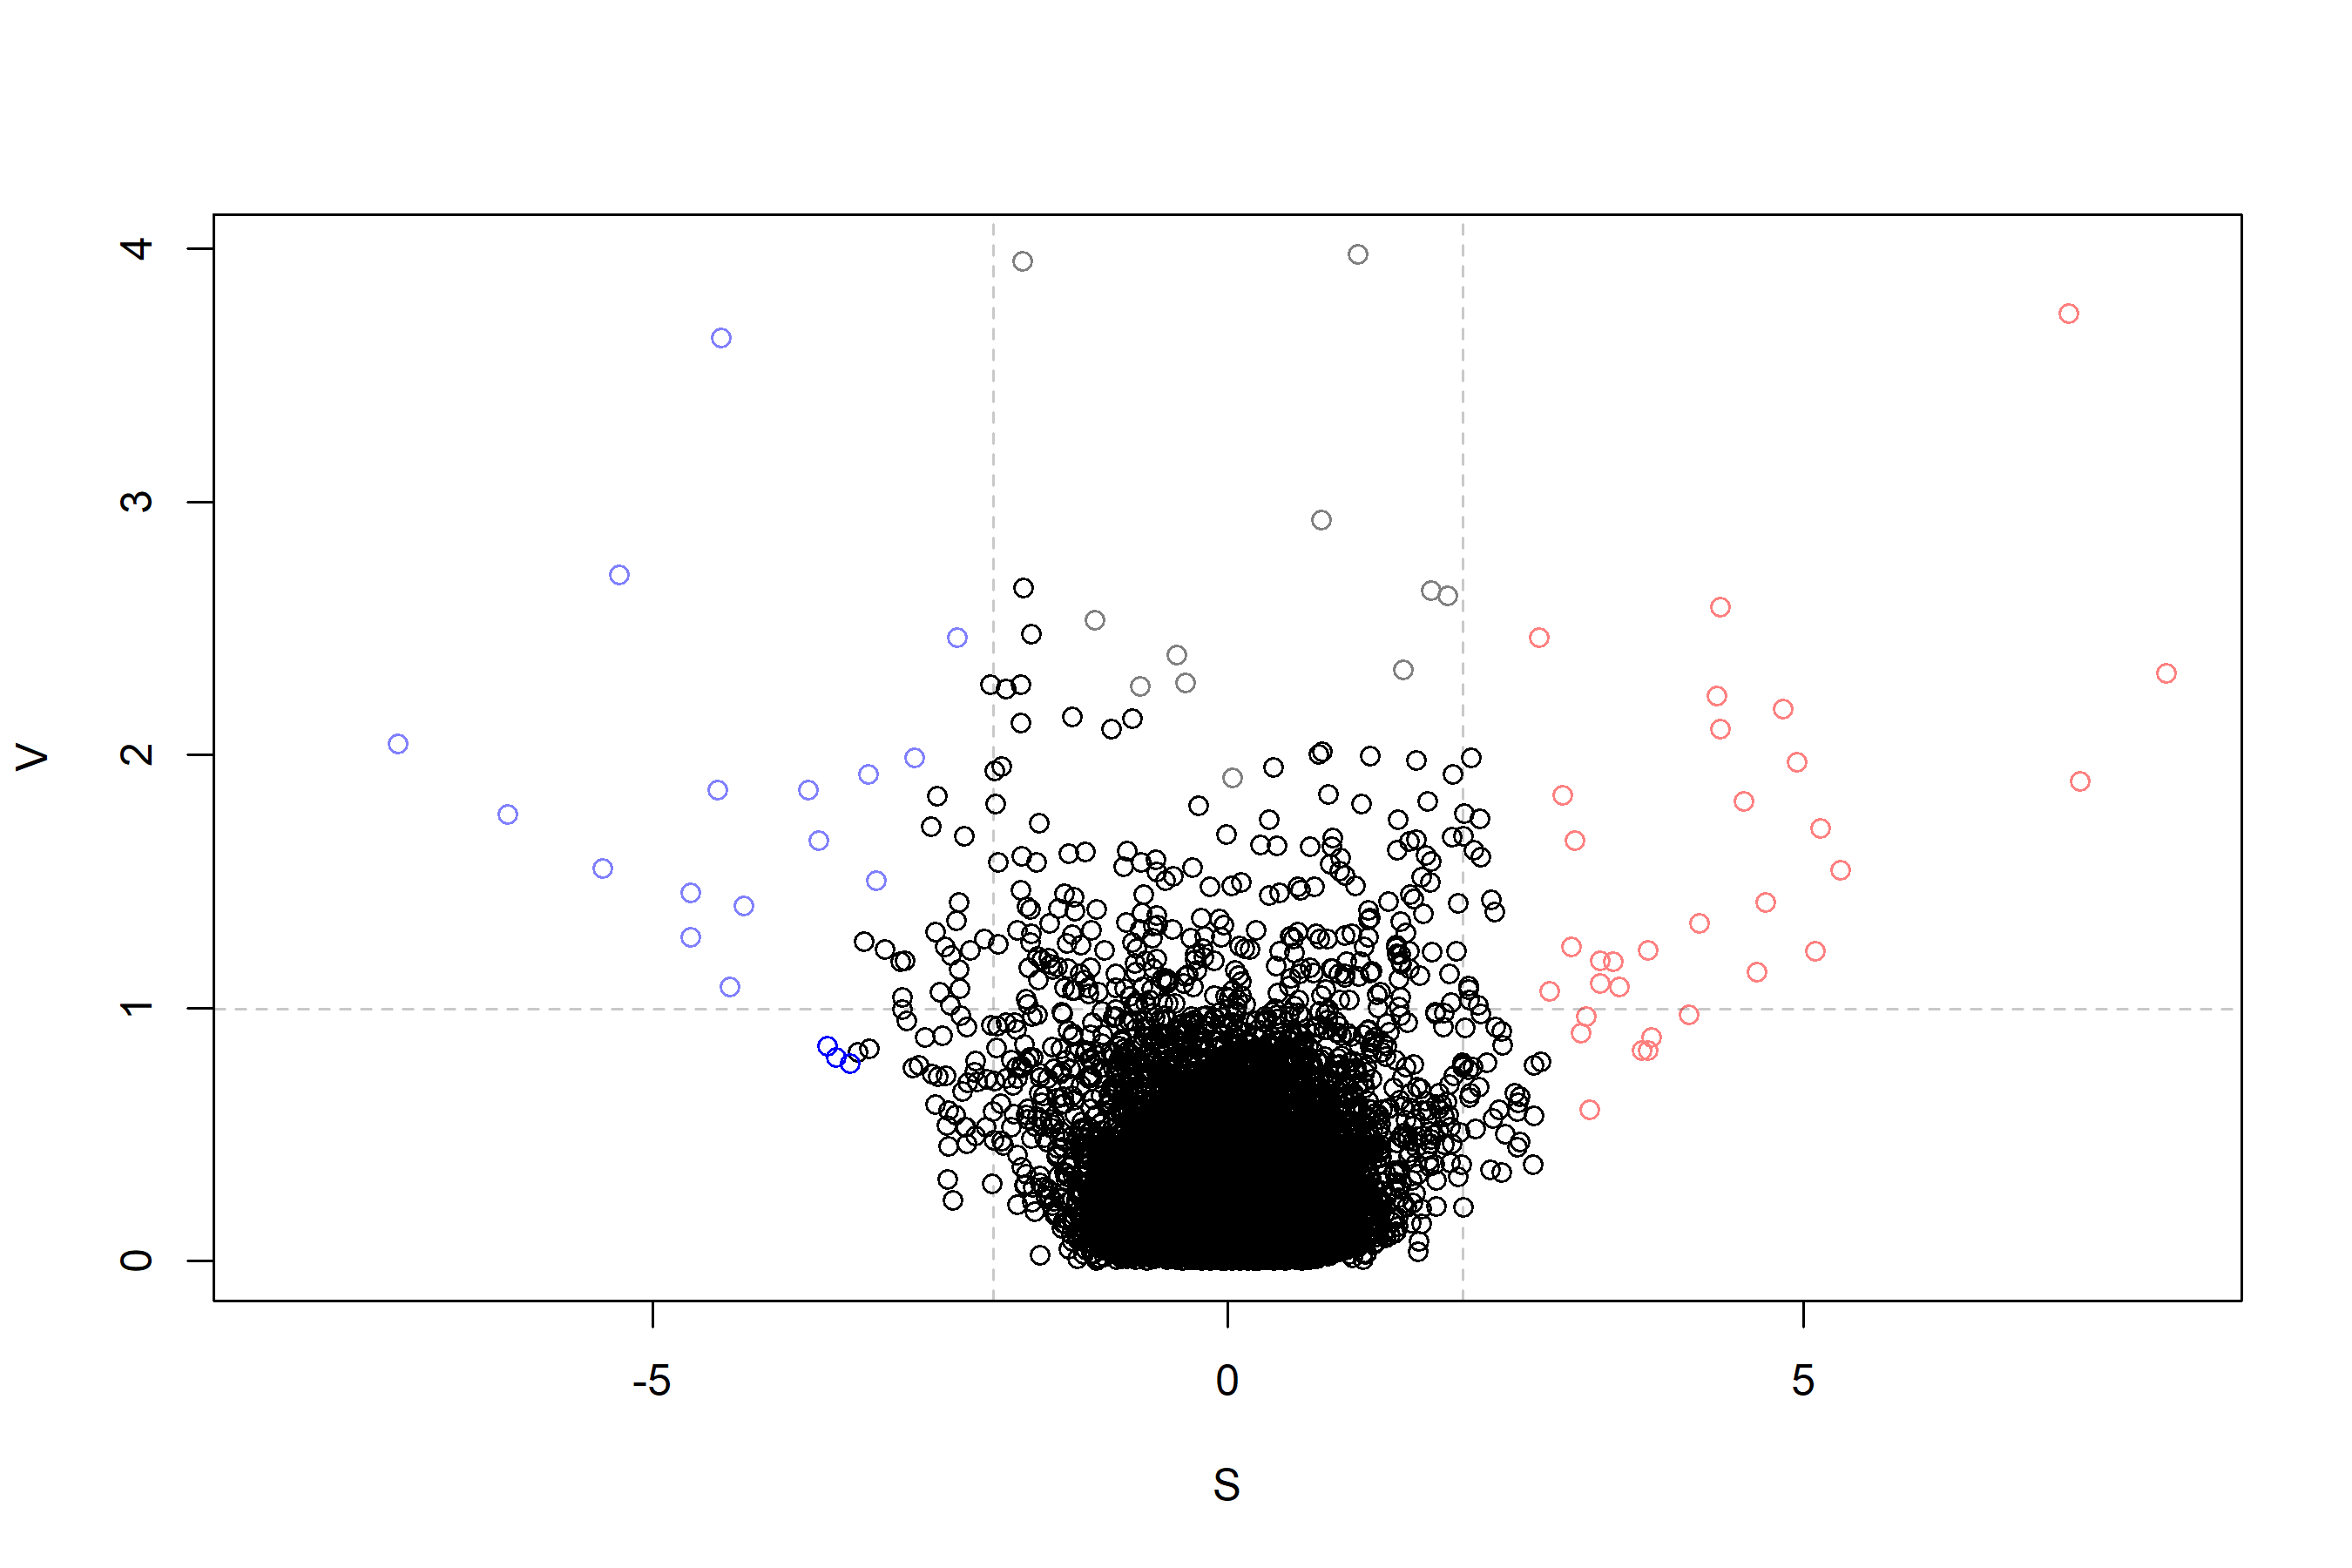
\includegraphics{README_files/figure-latex/unnamed-chunk-31-1.png}
\caption{SV-plot produced from a \texttt{GEVAResults} object using the
\texttt{geva.finalize} function with \texttt{0.05} as p-value cutoff.}
\end{figure}

\clearpage

\hypertarget{accessing-and-extracting-the-results}{%
\subsection{Accessing and extracting the
results}\label{accessing-and-extracting-the-results}}

The returned \texttt{GEVAResults} object from \texttt{geva.finalize}
represents the concatenation of all previous steps in addition to the
results table and, if applicable, the intermediate steps from the factor
analysis. The results table stores the final gene classifications,
including the relevant (\texttt{"similar"}, \texttt{"factor-dependent"},
and \texttt{"factor-specific"}) and irrelevant (\texttt{"sparse"} and
\texttt{"basal"}) ones. Each classification can be briefly described as
follows:

\begin{itemize}
\tightlist
\item
  \texttt{basal}: Genes with similar but mild \emph{logFC} that
  approximates to zero. Note that despite this name they not necessarily
  represent basal levels of gene expression, especially if the control
  group from DE analysis is not under normal conditions;
\item
  \texttt{sparse}: Genes with high \emph{logFC} variation but lacking
  any relationship to the experimental conditions or the factors;
\item
  \texttt{similar}: Genes with relevant \emph{logFC} (far from zero) and
  low \emph{logFC} variance;
\item
  \texttt{factor-dependent}: Genes with low \emph{logFC} variance within
  the specified factors, but high variance between diferent factors;
\item
  \texttt{factor-specific}: Genes with low \emph{logFC} variance within
  one specific factor.
\end{itemize}

The function \texttt{results.table} can be used to return the table of
final gene classifications:

\begin{Shaded}
\begin{Highlighting}[]
\KeywordTok{tail}\NormalTok{(}\KeywordTok{results.table}\NormalTok{(gresults), }\DecValTok{10}\NormalTok{)}
\end{Highlighting}
\end{Shaded}

\begin{longtable}[]{@{}lll@{}}
\toprule
& classification & specific.factor\tabularnewline
\midrule
\endhead
probe\_9991 & basal & NA\tabularnewline
probe\_9992 & basal & NA\tabularnewline
probe\_9993 & basal & NA\tabularnewline
probe\_9994 & basal & NA\tabularnewline
probe\_9995 & basal & NA\tabularnewline
probe\_9996 & basal & NA\tabularnewline
probe\_9997 & basal & NA\tabularnewline
probe\_9998 & factor-specific & Cond\_2\tabularnewline
probe\_9999 & basal & NA\tabularnewline
probe\_10000 & basal & NA\tabularnewline
\bottomrule
\end{longtable}

On the other hand, the \texttt{top.genes} function may be a rather
practical way to return the most relevant results. It extracts by
default the \texttt{"similar"}, \texttt{"factor-dependent"}, and
\texttt{"factor-specific"} results, and can attach additional columns
(\emph{e.g.}, gene symbols) specified by the \texttt{add.cols}
arguments. The code below shows an usage example of \texttt{top.genes}:

\begin{Shaded}
\begin{Highlighting}[]
\CommentTok{# Extracts the top genes only}
\NormalTok{dtgens <-}\StringTok{ }\KeywordTok{top.genes}\NormalTok{(gresults)}

\CommentTok{# Extracts the top genes and appends the "Symbol" column}
\NormalTok{dtgens <-}\StringTok{ }\KeywordTok{top.genes}\NormalTok{(gresults, }\DataTypeTok{add.cols =} \StringTok{"Symbol"}\NormalTok{)}

\CommentTok{# Prints the last lines of the top genes table (optional)}
\KeywordTok{print}\NormalTok{(}\KeywordTok{tail}\NormalTok{(dtgens, }\DecValTok{10}\NormalTok{))}
\end{Highlighting}
\end{Shaded}

\begin{longtable}[]{@{}llll@{}}
\toprule
& Symbol & classification & specific.factor\tabularnewline
\midrule
\endhead
probe\_8487 & GENE\_K8487 & factor-dependent & NA\tabularnewline
probe\_8740 & GENE\_D8740 & factor-dependent & NA\tabularnewline
probe\_8823 & GENE\_I8823 & factor-specific & Cond\_1\tabularnewline
probe\_9136 & GENE\_J9136 & similar & NA\tabularnewline
probe\_9312 & GENE\_D9312 & factor-dependent & NA\tabularnewline
probe\_9495 & GENE\_E9495 & factor-dependent & NA\tabularnewline
probe\_9601 & GENE\_G9601 & factor-specific & Cond\_3\tabularnewline
probe\_9758 & GENE\_H9758 & factor-specific & Cond\_3\tabularnewline
probe\_9893 & GENE\_M9893 & factor-dependent & NA\tabularnewline
probe\_9998 & GENE\_N9998 & factor-specific & Cond\_2\tabularnewline
\bottomrule
\end{longtable}

The resulting table can then be exported using functions such has
\texttt{write.table} from the R base package.

\hypertarget{shortcut-function-and-reanalysis}{%
\subsection{Shortcut function and
reanalysis}\label{shortcut-function-and-reanalysis}}

The \texttt{geva.quick} function accepts a \texttt{GEVAInput} object and
performs all intermediate functions from the summarization to the final
concatenation. Optional (\texttt{...}) arguments are passed to the
internal calls to \texttt{geva.summarize}, \texttt{geva.quantiles},
\texttt{geva.cluster} and \texttt{geva.finalize}, ultimately returning a
\texttt{GEVAResults} object. The basic usage is described as follows:

\begin{Shaded}
\begin{Highlighting}[]
\CommentTok{# Generates a random GEVAInput example}
\NormalTok{ginput <-}\StringTok{ }\KeywordTok{geva.ideal.example}\NormalTok{()}
\CommentTok{# Performs all intermediate steps with geva.quick}
\CommentTok{# The resolution is used by the call to geva.cluster}
\NormalTok{gresults <-}\StringTok{ }\KeywordTok{geva.quick}\NormalTok{(ginput, }\DataTypeTok{resolution=}\FloatTok{0.25}\NormalTok{)}
\CommentTok{## > Found 4 clusters and 31 significant genes}
\NormalTok{gresults <-}\StringTok{ }\KeywordTok{geva.quick}\NormalTok{(ginput, }\DataTypeTok{resolution=}\FloatTok{0.4}\NormalTok{)}
\CommentTok{## > Found 16 clusters and 116 significant genes}
\end{Highlighting}
\end{Shaded}

This function can be applied to a \texttt{GEVAResults} object as well to
restore the parameters that produced this result, whereas optional
(\texttt{...}) arguments can overwrite them:

\begin{Shaded}
\begin{Highlighting}[]
\CommentTok{# Generates a random GEVAInput example}
\NormalTok{ginput <-}\StringTok{ }\KeywordTok{geva.ideal.example}\NormalTok{()}
\CommentTok{# Performs all intermediate steps with geva.quick}
\CommentTok{# The summary.method is used by the call to geva.summarize}
\NormalTok{gresults <-}\StringTok{ }\KeywordTok{geva.quick}\NormalTok{(ginput, }\DataTypeTok{summary.method=}\StringTok{'mean'}\NormalTok{)}
\CommentTok{## > Found 60 significant genes}
\NormalTok{gresults <-}\StringTok{ }\KeywordTok{geva.quick}\NormalTok{(gresults, }\DataTypeTok{summary.method=}\StringTok{'median'}\NormalTok{)}
\CommentTok{## > Found 95 significant genes}
\end{Highlighting}
\end{Shaded}

In the example above, the entire analysis was redone using the
overwritten \texttt{summary.method} argument. Therefore, by following
this pattern, users can tweak different parameters depending on their
statistical choice regarding the current biological context.

\end{document}
